\chapter{Анализ одномерной модели пассивного электростатического подвеса} \label{chapt2}

\section{Исследование одномерного пассивного электрического подвеса с постоянным напряжением, анализ его устойчивости. Теорема Ирншоу} \label{sect2_1}

Рассмотрим конфигурацию электростатического подвеса состоящего из проводящей незаряженной пластинки, помещенной между обкладками плоского конденсатора (рис.~\ref{img:simple_susp_1}). Окажется, что тело в такой системе не имеет устойчивых положений равновесия, электрические силы не зависят от положения тела, а результирующая электрических сил обращается в ноль. Действительно, запишем выражение для энергии электрического поля:
\begin{equation}
  \label{eq:simple_susp_energy_1}
  W_e = \frac{e^2}{2C_1}+\frac{e^2}{2C_2}
\end{equation}

\noindent где $e$ – заряд на конденсаторе, $C_1 = \frac{\epsilon_0 S}{h-y}$ – емкость между верхним электродом и пластиной, $C_2 = \frac{\epsilon_0 S}{h+y}$ – емкость между пластиной и нижним электродом, $h$ – половина расстояния между электродами, $y$ – смещение пластины вдоль вертикальной оси из среднего положения.

Таким образом, энергия $W_e$ (\ref{eq:simple_susp_energy_1}) не зависит от положения пластины, и результирующая сила, действующая на пластину со стороны электрического поля обращается в нуль.

\begin{figure}[ht]
    {\centering
        \hfill
        \subbottom[List-of-Figures entry][Двухэлектродный электростатический подвес\label{img:simple_susp_1}]{%
            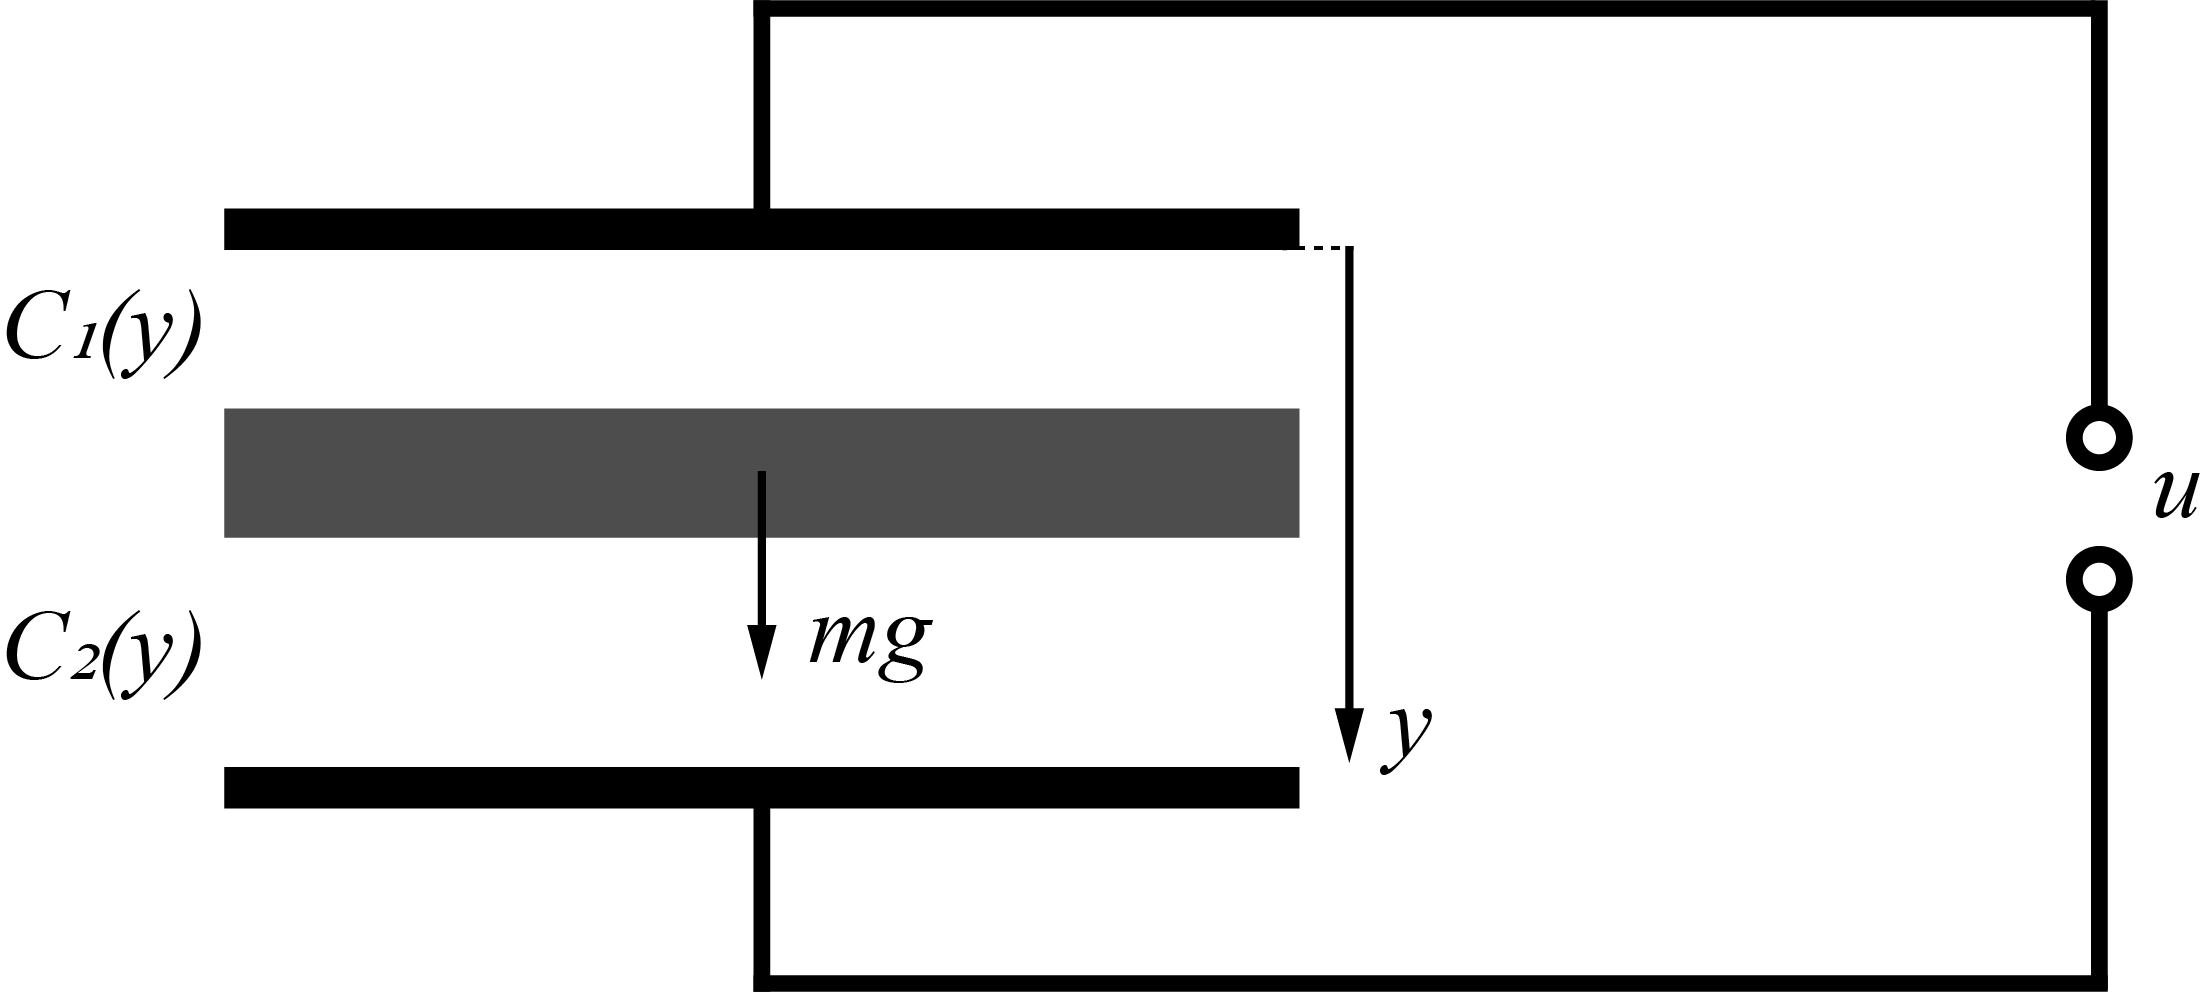
\includegraphics[width=0.49\linewidth]{simple_susp_1}}
        \hfill
        \subbottom[Четырехэлектродный электростатический подвес\label{img:simple_susp_2}]{%
            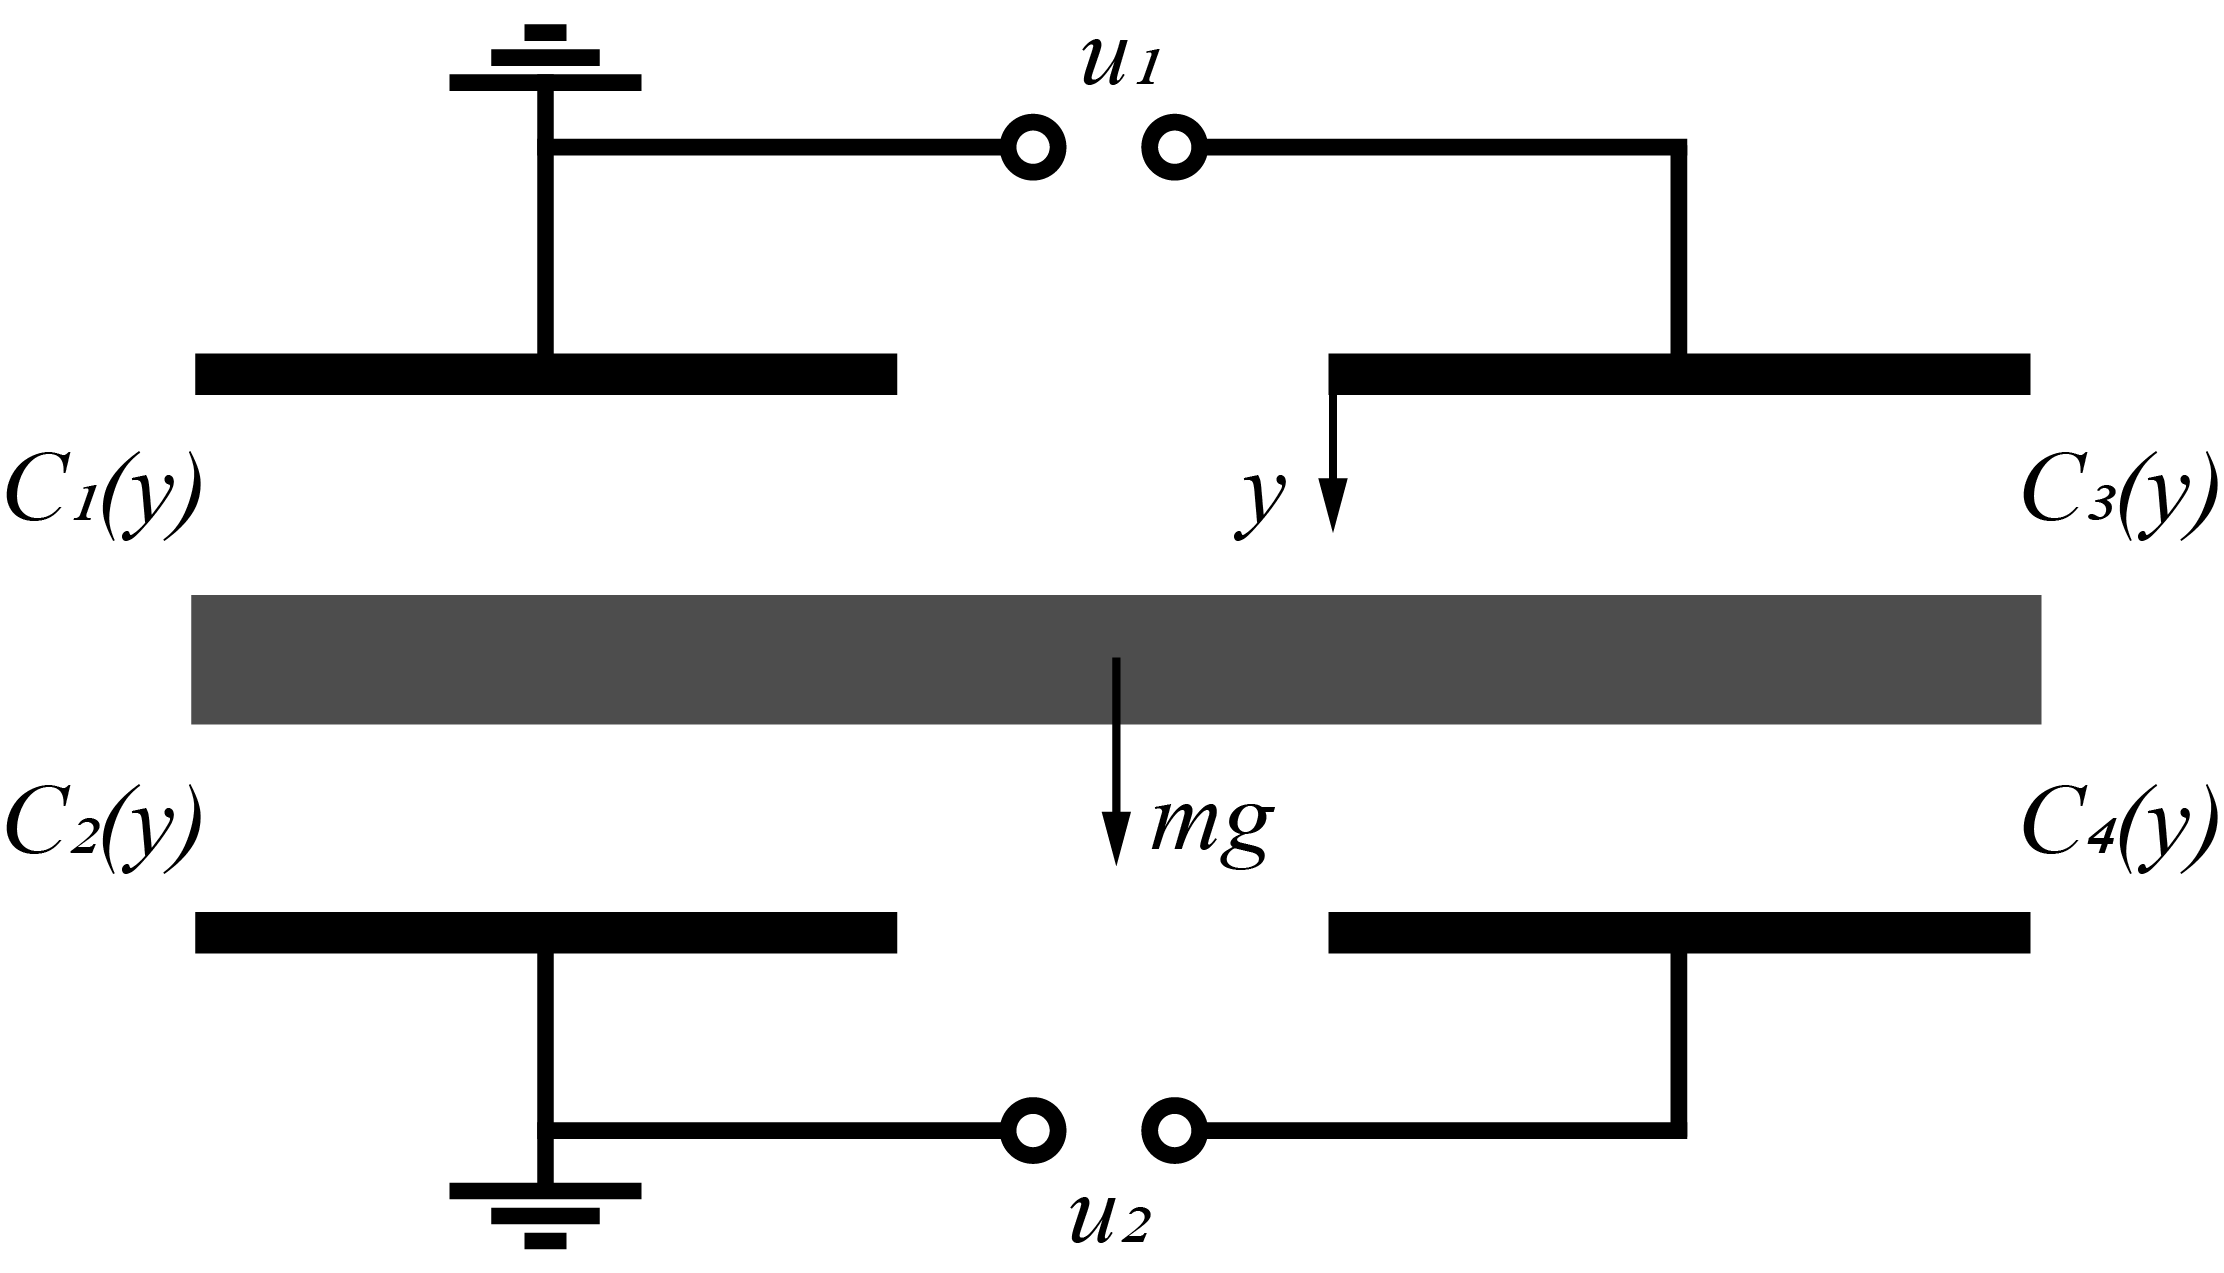
\includegraphics[width=0.49\linewidth]{simple_susp_2}}
        \hfill
    }
    \caption{Простейшие случаи электростатического подвеса}
    \label{img:simple_susp}
\end{figure}


Поэтому для создания одноосного электростатического подвеса незаряженного тела поместим его в электрическое поле созданное двумя парами электродов (рис. \ref{img:simple_susp_2}). Повторим процедуру и запишем уравнение энергии электрического поля для эквивалентной электрической схемы, изображенной на рис. \ref{img:simple_susp_equivalent}. Обозначим через $e_1$, $e_2$ заряды на конденсаторах $C_1$, $C_2$. Дифференцируя выражение энергии электрического поля, взятого с противоположным знаком, получим выражение для силы, действующей на твердое тело \cite{Martynenko}:

\begin{equation}
  \label{eq:simple_susp_energy_2}
  F(y) = \frac{\epsilon_0 S}{4} \left[\left( \frac{u_1}{h-y} \right)^2 - \left( \frac{u_2}{h+y} \right)^2\right],
\end{equation}

\noindent где $u_1$, $u_2$ – напряжения на электродах, связанные с зарядами на конденсаторах $e_1$ и $e_2$ соотношениями $u_1 = \frac{e_1}{C_1} + \frac{e_1+e_2}{C_3+C_4}$ и $u_2 = \frac{e_2}{C_2} + \frac{e_1+e_2}{C_3+C_4}$. 

\begin{figure}[ht] 
  \centering
  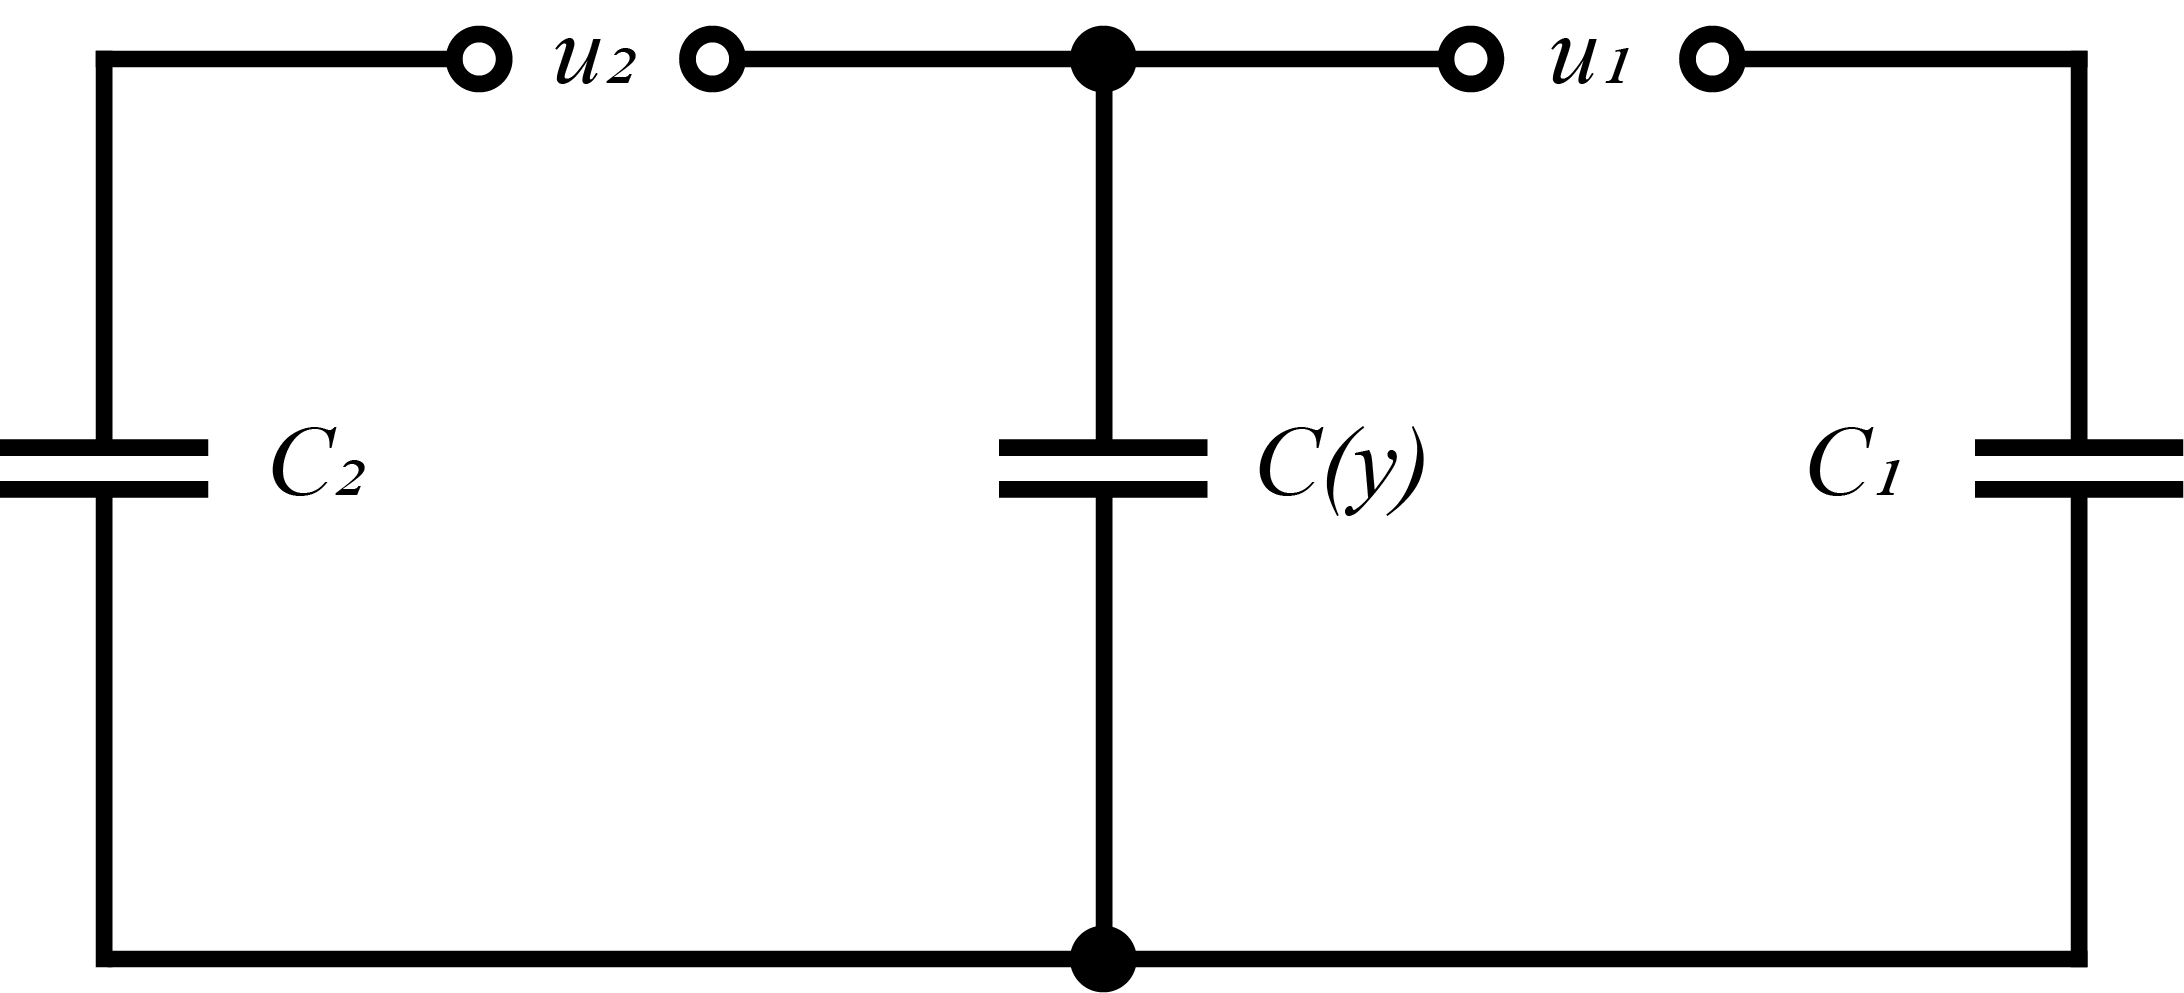
\includegraphics [scale=0.5] {simple_susp_equivalent}
  \caption{Эквивалентная электрическая схема четырехэлектродного электростатического подвеса}
  \label{img:simple_susp_equivalent}
\end{figure}

Функция $F(y)$ монотонно возрастает от $-\infty$ до $+\infty$ при $-h<y<h$. Положения равновесия тела в подвесе определяются из условия равенства веса тела $mg$ пондеромоторной силе $F$. На интервале $(-h, h)$ уравнение $F(y)=mg$ имеет единственное решение, потенциальная энергия при этом будет иметь максимум, а положение равновесия будет неустойчивым.

Данная ситуация является следствием теоремы Ирншоу о неустойчивости электрических систем \cite[с.~92]{Tamm}, которая говорит о том, что нахождение проводящего тела в состоянии устойчивого равновесия в электрическом поле под действием только электрических сил невозможно.


%\newpage
%============================================================================================================================

\section{Исследование одномерного пассивного электростатического подвеса с переменным напряжением} \label{sect2_2}

\subsection{Методы стабилизации тела в электростатическом подвесе. Простейшие системы управления, доставляющие асимптотическую устойчивость положению равновесия} \label{subsect2_2_1}

\begin{figure}[ht] 
  \centering
  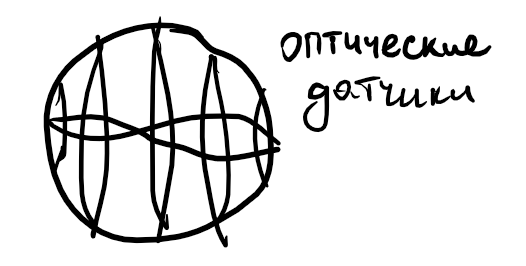
\includegraphics [scale=1.0] {optical_sensors}
  \caption{Рисунок на роторе сферического гироскопа для фиксации положения оптическим датчиком}
  \label{img:optical_sensors}
\end{figure}

Для создания устойчивого положения равновесия твердого тела в электростатическом подвесе необходимо управление потенциалами электродов. Обычно положение твердого тела в электростатическом подвесе измеряется специальными датчикам (емкостными или оптическими, рис. \ref{img:optical_sensors}) \cite{Electropribor}. Электростатические подвесы с системами слежения, то есть такие, напряжения на электродах которых изменяются в зависимости от положения тела, называют активными. Простейшую функцию пондеромоторных сил в активной системе можно представить в виде нелинейного закона управления:
\begin{equation}
  \label{eq:simple_susp_active_force}
  F(y) = \left\{
    \begin{alignedat}{2}
        &F_1(y), \quad &\text{eсли }& -h\geqslant y \geqslant -\frac{V}{k}, \\
        &F_2(y), \quad &\text{eсли }& -\frac{V}{k}\geqslant y \geqslant \frac{V}{k}, \\
        &F_3(y), \quad &\text{eсли }& \frac{V}{k}\geqslant y \geqslant -h,
    \end{alignedat}
    \right.
\end{equation}

\noindent где $V$ – некоторое постоянное «опорное» напряжение, $k$ – коэффициент усиления следящей системы, причем предполагается, что $k>V/h$. При $k>V/h$ график функции $F(y)$ построен на рис. \ref{img:active_susp_force_plot}.
Напряжения на электродах в таких системах могут быть не только функциями координаты смещения твердого тела, но и зависеть от его скорости, что позволяет исключить негативное влияние наличия запаздывания в следящей системе. Так как в действительности в соотношения $F(y)$ войдет значение координаты $y$, зависящей от некоторого предыдущего момента времени, что приведет к нарастанию амплитуды колебаний тела. 

\begin{figure}[ht] 
  \centering
  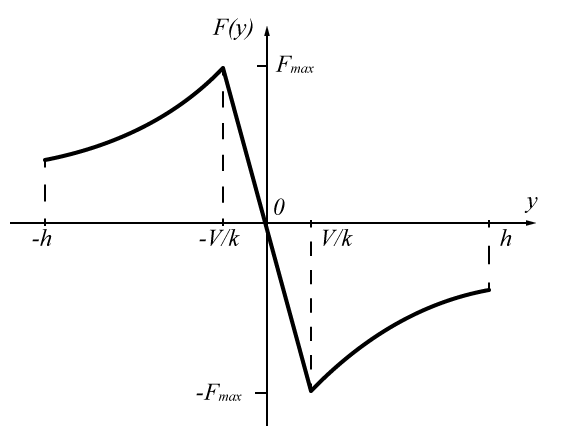
\includegraphics [scale=0.5] {active_susp_force_plot}
  \caption{Зависимость силы $F$ от смещения $y$ в активном электростатическом подвесе}
  \label{img:active_susp_force_plot}
\end{figure}

\subsection{Аналитическое исследование одноосного пассивного электростатического подвеса} \label{subsect2_2_2}

Справится с естественной неустойчивостью электростатических подвесов без использования активных следящих систем позволяют, например, пассивные или резонансные подвесы. Простейшая схема одноосного пассивного электростатического подвеса представлена на рисунке \ref{img:pas_susp_scheme}. Верхняя пластина плоского конденсатора является неподвижной, а нижняя пластина должна удерживаться на некотором расстоянии от верхней пластины в положении, когда вес пластины уравновешивается силой притяжения, действующей на проводник в электрическом поле, созданном между обкладками конденсатора.

Электрическая цепь рассматриваемой электромеханической системы образована индуктивностью $L$, конденсатором $C$, омическим сопротивлением $R$. ЭДС внешнего источника, подключенного к цепи, изменяется по синусоидальному закону $u = u_0 \sin \omega t$, $u_0$ – амплитуда, $\omega$ – частота.

\begin{figure}[ht] 
  \centering
  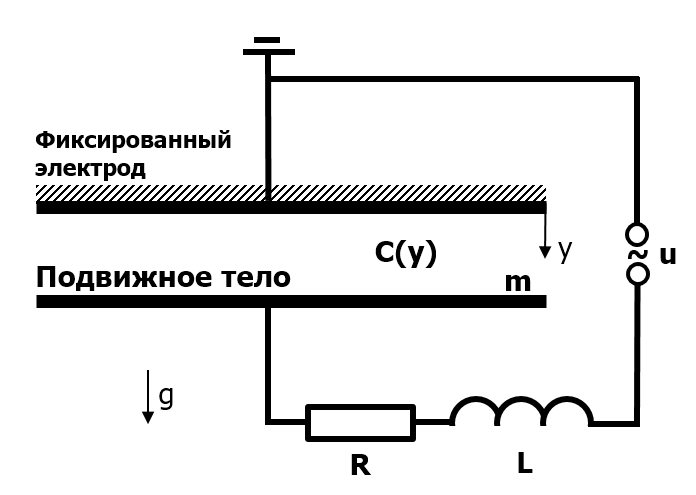
\includegraphics [scale=0.5] {pas_susp_scheme}
  \caption{Схема одноосного пассивного электростатического подвеса}
  \label{img:pas_susp_scheme}
\end{figure}

Запишем уравнения движения данной схемы, для этого обозначим через $m$ массу подвижной пластины и введем вертикальную ось $y$. Выберем начало отсчета в точке $O$, принадлежащей верхнему фиксированному электроду, тогда в реальной системе координата нижней пластины $y<0$.
В качестве обобщенных координат выберем координату $y$ подвижной пластины и заряд на конденсаторе $C(y) = \epsilon_0 S/y$. Кинетическая энергия пластины $T = m \dot y^2/2$, потенциальная энергия силы тяжести $\Pi = mgy$. Магнитная энергия электрической цепи $W_m=L \dot e^2/2$, где $\dot e \equiv i$ – ток в цепи. Энергия электрического поля, локализованного между обкладками конденсатора, без учета краевых эффектов
\[
W_e = \frac{e^2}{2C(y)} = - \frac{e^2 y}{2 \epsilon_0 S}.
\]

Функция Лагранжа для рассматриваемой электромеханической системы принимает вид
\[
L = T - \Pi + W_m - W_e = \frac{1}{2}m \dot y^2 - mgy + \frac{1}{2}L_1 \dot e^2 + \frac{e^2 y}{2 \epsilon_0 S}.
\]

Пластина подвешена в вакууме, силой трения при движении пластины пренебрегаем. Тогда диссипативная функция Рэлея будет определятся только потерями в электрической цепи $\Psi = \frac{1}{2}R \dot e^2$. Учитывая, что обобщенные неконсервативные силы механической природы отсутствуют, запишем уравнения Лагранжа–Максвелла \cite{Martynenko_andyn}
\[
\frac{d}{dt} \left( \frac{\partial L}{\partial \dot e} \right) - \frac{\partial L}{\partial e} + \frac{\partial \Psi}{\partial \dot e} = u, \quad
\frac{d}{dt} \left( \frac{\partial L}{\partial \dot y} \right) - \frac{\partial L}{\partial y} + \frac{\partial \Psi}{\partial \dot y} = 0.
\]

Выполняя операции дифференцирования, получаем уравнения движения
\begin{equation}
  \label{eq:pas_susp_motion}
    \begin{alignedat}{2}
    &L \ddot e + R \dot e - \frac{e y}{\epsilon_0 S} = u \sin \omega t, \\
    &m \ddot y + m g - \frac{e^2}{2 \epsilon_0 S} = 0.
    \end{alignedat}
\end{equation}

Система уравнений (\ref{eq:pas_susp_motion}) представляет систему нелинейных неавтономных дифференциальных уравнений 4-го порядка относительно переменных $y, e$, нахождение аналитического решения этой системы не представляется возможным.
Построим приближенное решение системы (\ref{eq:pas_susp_motion}), приняв $y$ в первом уравнении за постоянный параметр. Такое предположение возможно в силу того, что в реальных системах частота задающего напряжение $\omega$  велика по сравнению с механическими колебаниями $y$. В таком случае, первое уравнение системы (\ref{eq:pas_susp_motion}) принимает вид линейного дифференциального уравнения с постоянными коэффициентами. Решение данного уравнения представляет собой сумму общего и частного решений \cite{Martynenko}
\begin{equation}
  \label{eq:pas_susp_charge}
    e = \frac{u_0 \sin (\omega t + \phi)}{\sqrt{\left(L \omega^2 + \frac{y}{\epsilon_0 S} \right)^2 
    + \left( R \omega \right)^2}} + e_{\text{общ}},
\end{equation}

\noindent где $\phi$ – сдвиг по фазе между вынужденным колебанием и внешней силой, $e_{\text{общ}}$ – общее решение однородного уравнения, т.е. решение первого уравнения (\ref{eq:pas_susp_motion}) при $u_0=0$. Вне малого начального интервала времени общее решение $e_{\text{общ}}$ в силу того, что оно является экспоненциально убывающей функцией времени, можно считать равным нулю. Подставим (\ref{eq:pas_susp_charge}) во второе уравнение (\ref{eq:pas_susp_motion}) и заменим функцию $\sin{\omega t + \phi}^2$ его средним значением, тогда получим нелинейное дифференциальное уравнение второго порядка относительно переменной $y$
\begin{equation}
  \label{eq:pas_susp_sol_1}
    m \ddot y +mg -f(y)=0, \quad f(y) = \frac{1}{2 \epsilon_0 S} \frac{u_0^2}{\left(L \omega^2 + \frac{1}{\epsilon_0 S} y \right)^2 
    + \left( R \omega \right)^2}.
\end{equation}

Построим график функции $f(y)$ (рис. \ref{img:pas_susp_force_theory}). Функция $f(y)$ на интервале $-\infty < y < -L \epsilon_0 S \omega^2 $ возрастает от нуля до некоторого положительного значения, а затем при $-L \epsilon_0 S \omega^2 < y < 0 $ функция монотонно убывает. Для определения положений равновесия  положим $\ddot y =0$, тогда $mg = f(y)$ – уравнение для определения равновесных положений твердого тела в электростатическом подвесе.

\begin{figure}[ht] 
  \centering
  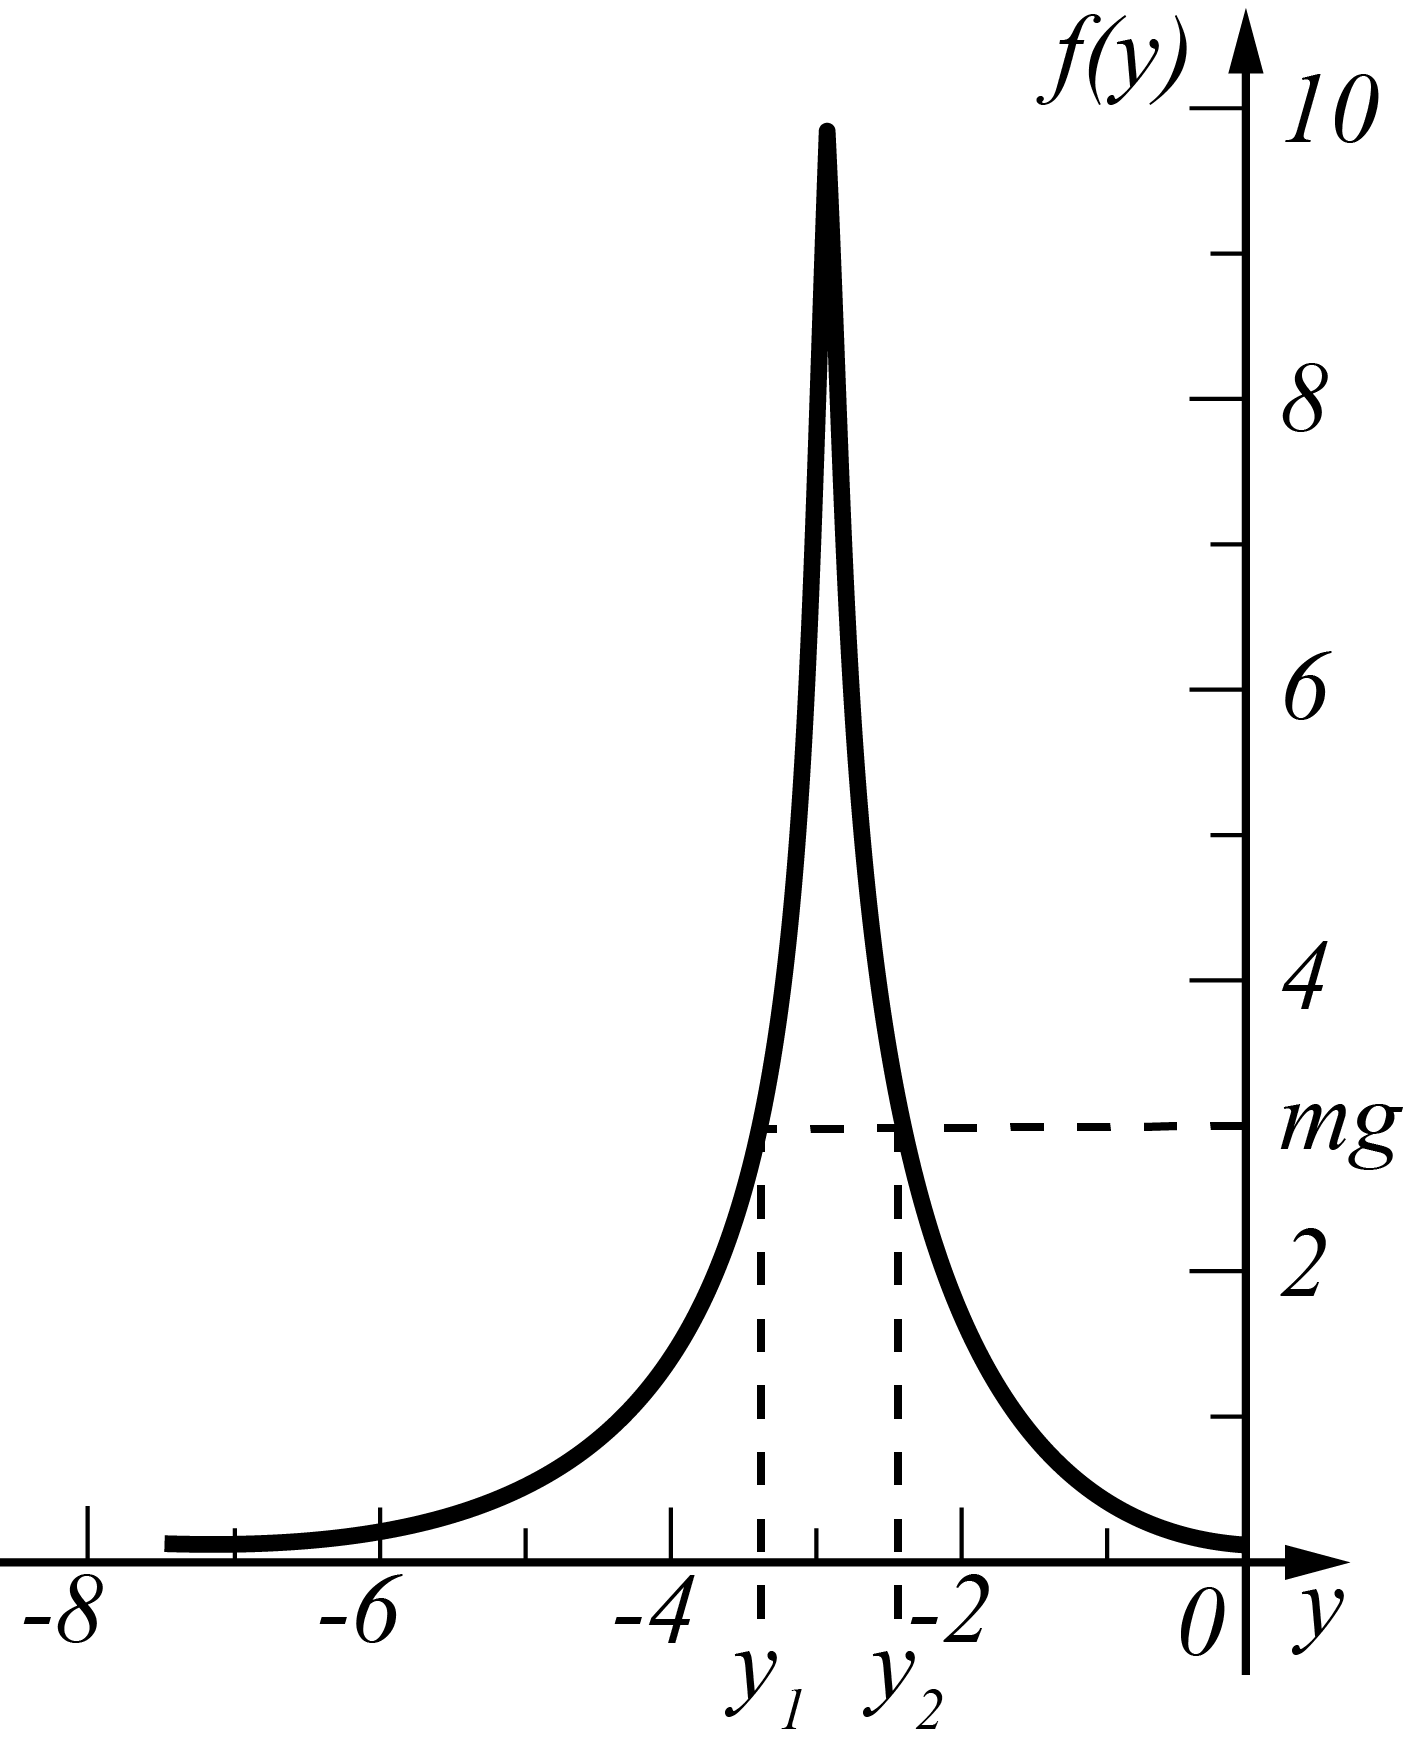
\includegraphics [scale=1] {pas_susp_force_theory}
  \caption{График функции $f(y)$}
  \label{img:pas_susp_force_theory}
\end{figure}

Максимальное значение функции $f_{max} = \frac{u_0^2}{4 \epsilon_0 S (R \omega)^2}$ отвечает за максимальный вес твердого тела, который способен удержать электростатический подвес. Будем считать, что $mg<f_{max}$. Тогда прямая $mg$ на рис. \ref{img:pas_susp_force_theory} пересекает $f(y)$ в двух точках $y=y_1, y=y_2$. В этом случае электростатический подвес имеет два положения равновесия.


Потенциальная энергия имеет вид (\ref{eq:pas_susp_potential}), ее график представлен на рис.  \ref{img:pas_susp_potential}. По теореме Лагранжа–Дирихле устойчивым оказывается положение равновесия $y = y_2$, положение равновесия $y=y_1$ неустойчиво.

\begin{equation}
  \label{eq:pas_susp_potential}
    \ddot y + \frac{\partial \Pi}{\partial y} = 0, \quad 
    \Pi(y) = gy - \frac{u_0^2}{4R m \omega} \arctan{ \frac{L \omega^2 + \frac{y}{\epsilon_0 S}}{R\omega} }
\end{equation}

\begin{figure}[ht] 
  \centering
  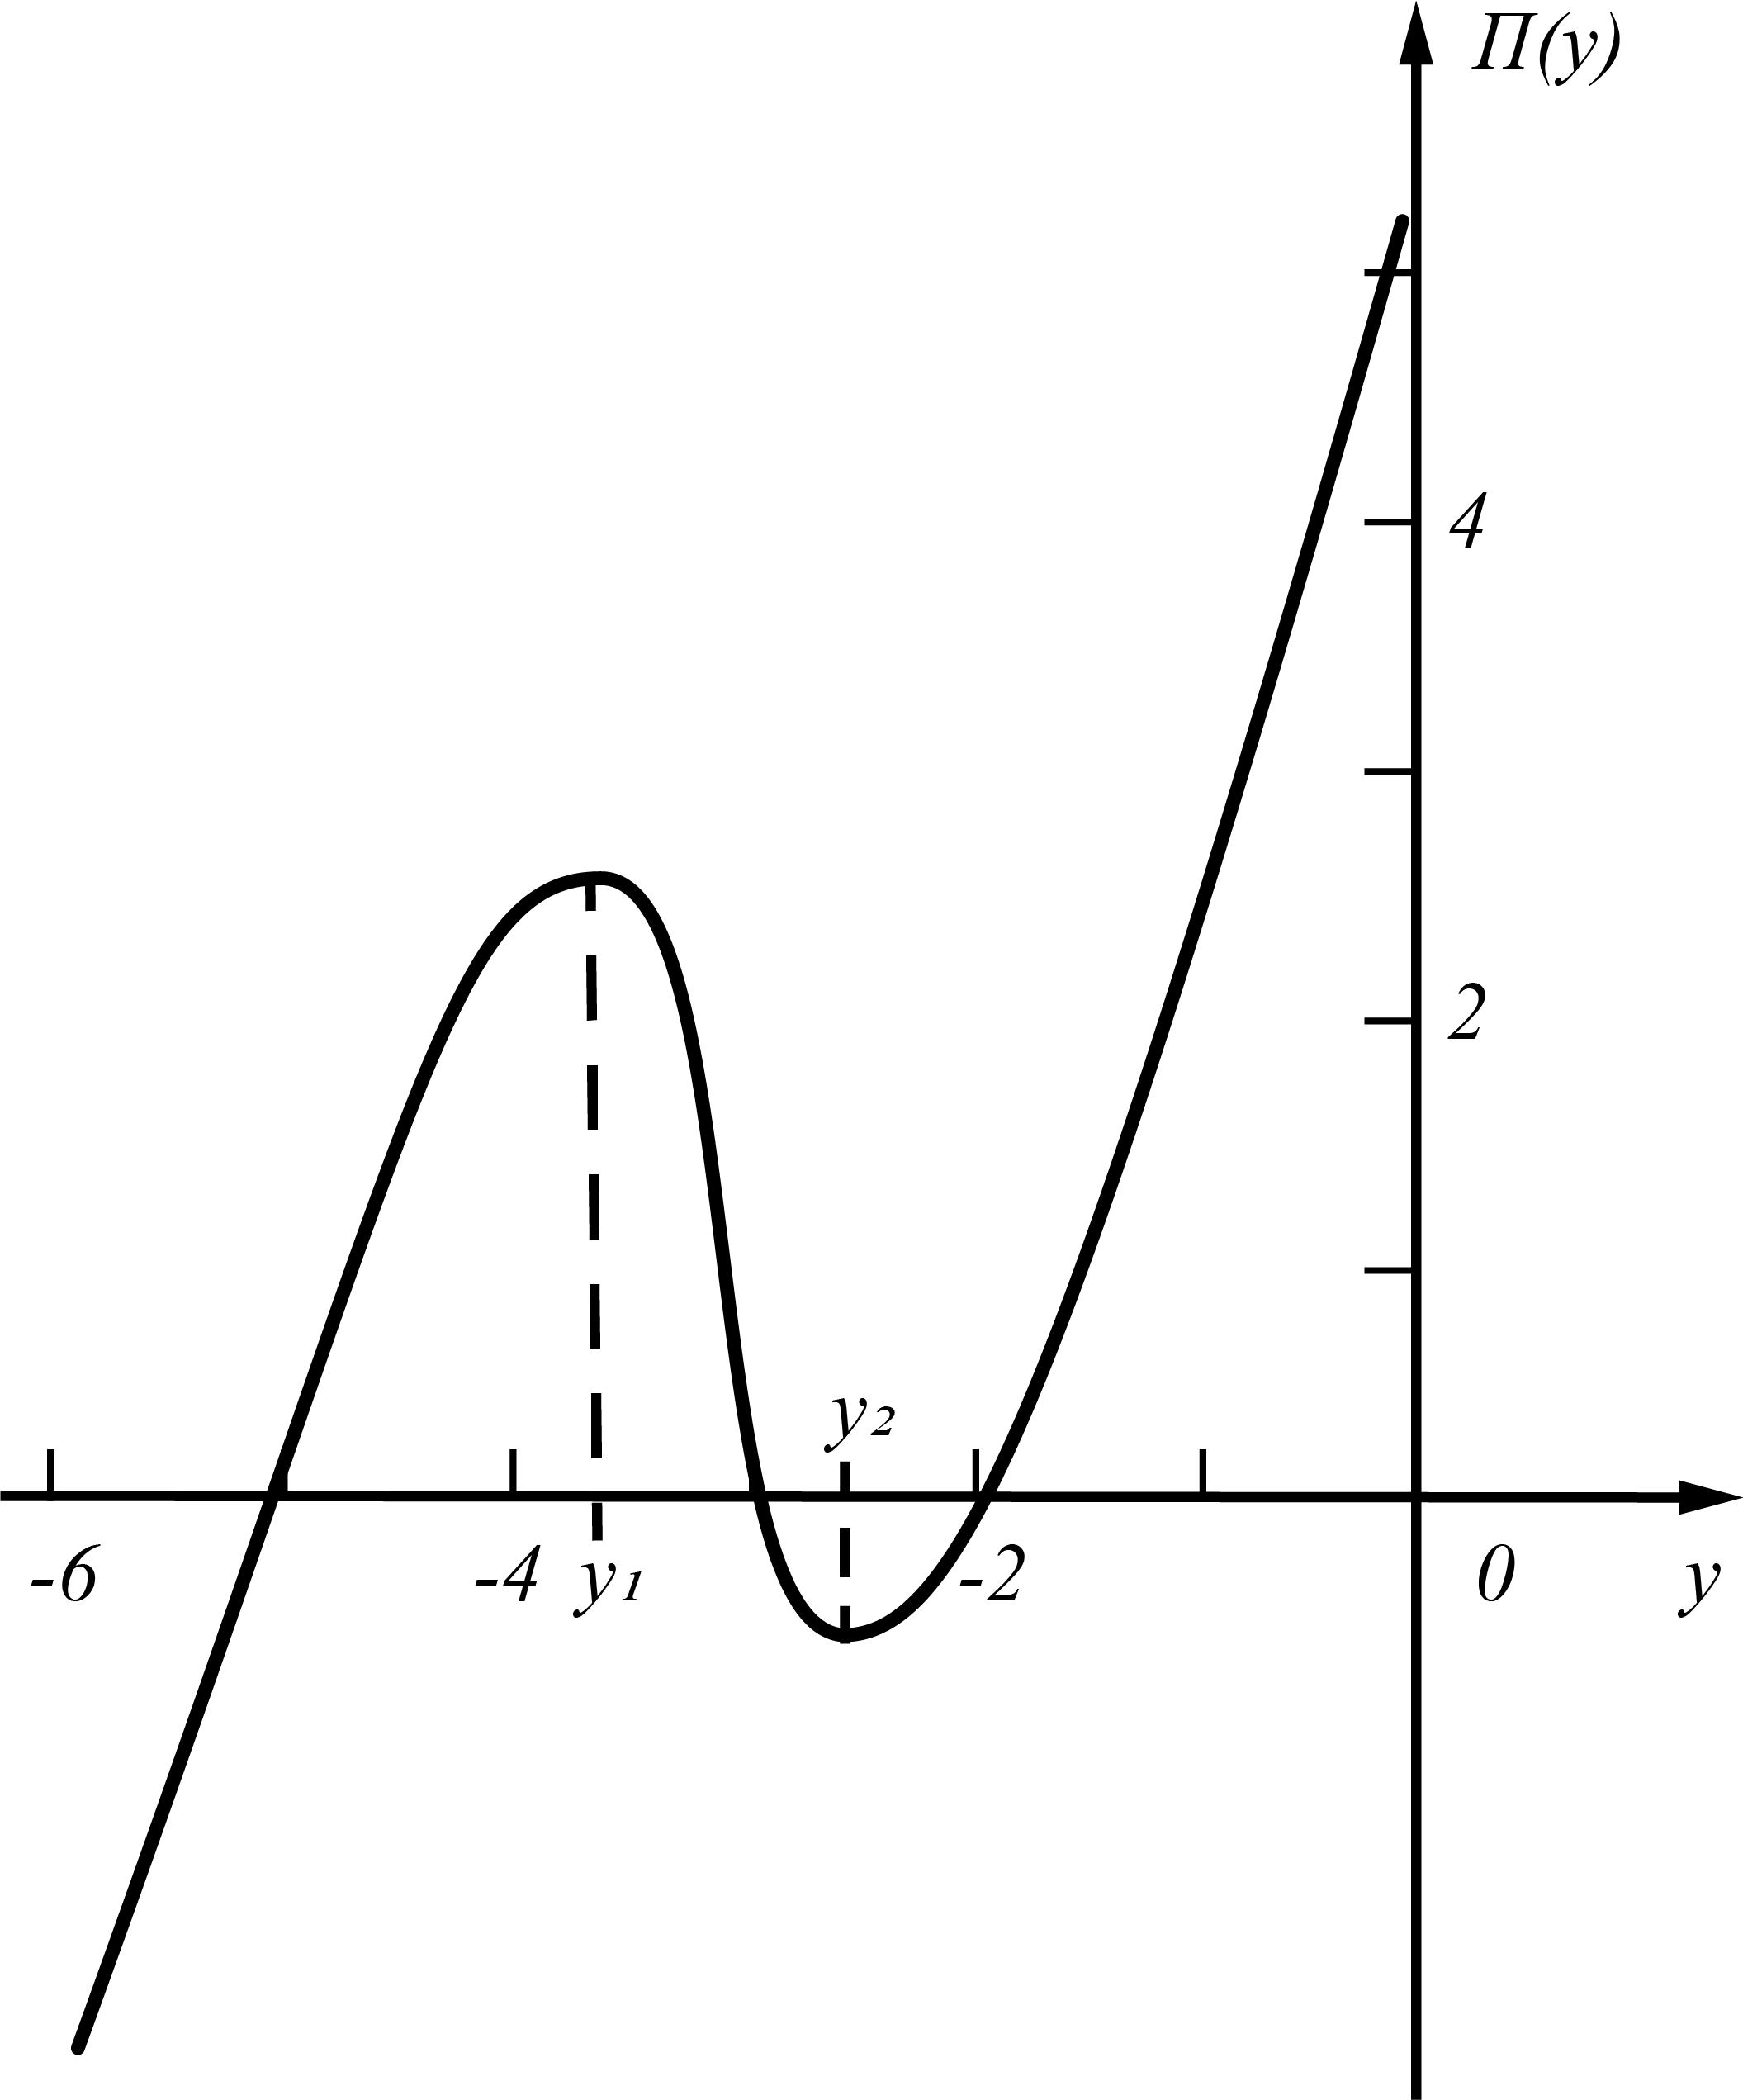
\includegraphics [scale=1] {pas_susp_potential}
  \caption{График функции $\Pi(y)$}
  \label{img:pas_susp_potential}
\end{figure}

\subsection{Обзор возможностей программной системы ANSYS для решения задач электромеханики. Методы определения пондеромоторных усилий в подвесах с применением численных решений ANSYS} \label{subsect2_3_2}

Программная система конечно-элементного анализа ANSYS предоставляет возможность моделирования электромеханических задач несколькими способами \cite{Ansys_coupled_field}:
\begin{enumerate}
  \item Прямое решение связанной задачи (Direct coupled-field analysis)
  \item Использование элементов преобразователей \textit{TRANS126} (Transducer elements)
  \item Параллельное решение двух связанных задач (Multi-field analysis)
  \item Прямое разложение по собственным формам (Reduced order modelling)
\end{enumerate}


\textbf{Прямое решение связной задачи} (Direct coupled-field analysis) реализуется благодаря совмещению в одном конечном элементе как трансляционных, так и электрических степеней свободы. Метод позволяет решать задачу в один шаг по времени, не разделяя электрическую и механическую задачи, более того, сочетание трансляционной и электрической степеней свободы позволяет учитывать неоднородности моделируемого электрического поля за счет геометрии конечных элементов.

Недостатками данного способа решения являются необходимость в случае сложной геометрии межэлектродного пространства использовать большое количество конечных элементов, несимметричность общей матрицы, приводящая к увеличению времени счета.

Метод предполагает использование специальных конечных элементов, например, двумерных квадратичных 8-ми узловых элементов \textit{PLANE223} или трехмерных квадратичных 12-ти узловых \textit{SOLID226}. Каждый узел элемента данных типов может содержать до 5 степеней свободы. Для решения связанной электромеханической задачи выберем электроупругую опцию элемента \textit{KEYOPT(1)=1001}, тогда каждый узел будет иметь 3 трансляционных и одну электрическую степени свободы: UX, UY, UZ, VOLT.


\textbf{Элементы преобразователи \textit{TRANS126}} представляют собой одномерные двух-узловые элементы с двумя степенями свободы в каждом узле: трансляционной (на выбор: UX, UY или UZ) и электрической (VOLT), Элементы данного типа предназначены для преобразования электрической энергии в механическую и наоборот, таким образом, позволяют связать электрические и механические степени свободы. 

Принцип работы заключается в наличии в элементе зависимости электрической емкости $C$ от зазора $\delta$ между его узлами
\[
C = C(\delta), \quad \delta = \delta_0 +u_1 - u_2,
\]
\noindent где $\delta_0$ – начальный зазор, $u_1, u_2$ – координаты $1$-го и $2$-го узлов элемента соответственно.

Существует возможность задания зависимости $C(\delta)$ как в форме полинома 4-ой степени, так и парами чисел «емкость–зазор». Расчет зависимости $C(\delta)$ производится предварительно отдельным расчетом, например, с помощью макроса \textit{CMATRIX} \cite[с.~275]{Ansys_command_reference}. Таким образом, в элементах–преобразователях рассчитывается зависимость электрической силы от положения тела. Появляется возможность схематизировать сложное электрическое поле совокупностью конечного числа элементов–преобразователей (рис. \ref{img:multi_trans126}).

\begin{figure}[ht] 
  \centering
  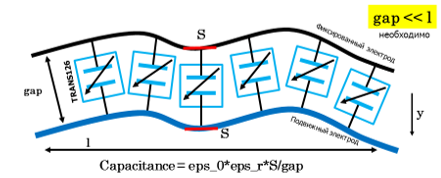
\includegraphics [scale=1] {multi_trans126}
  \caption{Пример схематизации электрического поля множеством элементов–преобразователей \textit{TRANS126}}
  \label{img:multi_trans126}
\end{figure}


Преимуществами данного метода являются простота построения конечно-элементной модели, малое расчетное время, а также возможность учета механического контакта пластин конденсатора. Вынужденная схематизация электрического поля является одним из недостатков метода, не позволяющая учитывать неоднородности электрического поля.



В данной работе не уделено внимание подробному рассмотрению методов \textbf{параллельного решения связанных задач} (Multi-Field analysis) и \textbf{прямого разложения по собственным формам} (Reduced order modelling). Отметим лишь, что принцип работы первого строится на итерационном решении механической и электрической задач, значения усилий и перемещений в данном методе интерполируются между несвязанными моделями. Основным недостатком такого подхода является необходимость перестраивания сетки на каждом итерационном шаге, что негативно отражается на времени счета. Метод прямого разложения, как следует из названия, основывается на разложении электромеханической задачи по собственным формам. Отличительной чертой метода является его эффективность при решении динамических задач на больших промежутках времени. Оба метода подробно описаны в \cite{Ansys_coupled_field}.


\subsection{Конечно-элементное моделирование и анализ одномерного пассивного электростатического подвеса с переменным напряжением} \label{subsect2_2_3}

Аналитическое исследование одноосного пассивного электростатического подвеса проведено ранее в разделе \ref{subsect2_2_1}. Для получения численных оценок поведения подвеса обратимся к возможностям конечно-элементной программной системы ANSYS Mechanical, которые были разобраны в предыдущем разделе \ref{subsect2_2_2}.

\begin{figure}[ht] 
  \centering
  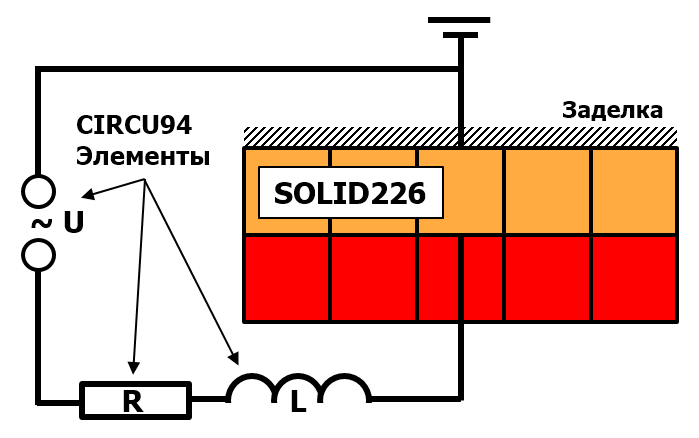
\includegraphics [scale=0.5] {pas_susp_solid226_scheme}
  \caption{Расчетная схема конечно-элементной постановки методом прямого решения связанной задачи}
  \label{img:pas_susp_solid226_scheme}
\end{figure}

Построим расчетную конечно-элементную модель для прямого решения связанной задачи. Элементами \textit{SOLID226} моделируем пространство между электродом и твердым телом электростатического пассивного подвеса (рис. \ref{img:pas_susp_scheme}). На узлы, принадлежащие верхнему электроду, задаем связь равенства между собой электрических VOLT и трансляционных UX, UY, UZ степеней свободы (\textit{Coupling}–связь), ту же связь задаем и на узлы соответствующие твердому телу. Помимо этого, на узлы, принадлежащие поверхности твердого тела, применяем граничное условие первого рода VOLT $=0$. Массу твердого тела моделируем $MASS21$ элементом. Разность потенциалов на противоположных гранях получившегося объема, т.е. разность потенциалов между электродом и телом, порождают в узлах силы, эквивалентные пондеромоторным электрическим силам, связывая тем самым механическую и электрическую задачи. Электрическую цепь моделируем одномерными элементами \textit{CIRCU94}, содержащими одну электрическую степень свободы VOLT. Схема расчетной модели для метода прямого решения связанной задачи с использованием \textit{SOLID226} элементов представлена на рис. \ref{img:pas_susp_solid226_scheme}.

Выбор параметров системы проводим на основе аналитических оценок раздела \ref{subsect2_2_1}. Для моделирования одноосного пассивного подвеса методом конечных элементов с использованием метода прямого решения связанной задачи приняты следующие параметры:

\begin{itemize}
  \item Амплитуда источника напряжения $u_0 = 10\ \text{В}$
  \item Частота источника напряжения $\omega = 40\ \text{кГЦ}$
  \item Сопротивление резистора $R = 300\ \text{Ом}$
  \item Индуктивность $L = 2\ \text{мГн}$
  \item Номинальный зазор $\delta_0 = 3\ \text{мкм}$
  \item Масса удерживаемого твердого тела $m = 6.25\ \text{г}$
  \item Площадь фиксированного электрода $S = 50\ \text{см}^2$
\end{itemize}

В силу большого времени счета ограничимся решением динамической задачи данным методом с фиксированным твердым телом, т.~е. при $y = const = \delta_0$. 

Решение производим путем динамического конечно-элементного анализа \textit{(ANTYPE,TRANS)} методом Ньютона-Рафсона (модифицированный метод касательных) \cite{Ansys_theory_reference}, шаг интегрирования задаем вручную, для этого проанализируем сходимость численного конечно-элементного решения, построив график зависимости значения напряжения на верхнем электроде от величины шага интегрирования (рис. \ref{img:pas_susp_solid226_conv}). 


\begin{figure}[ht] 
  \centering
  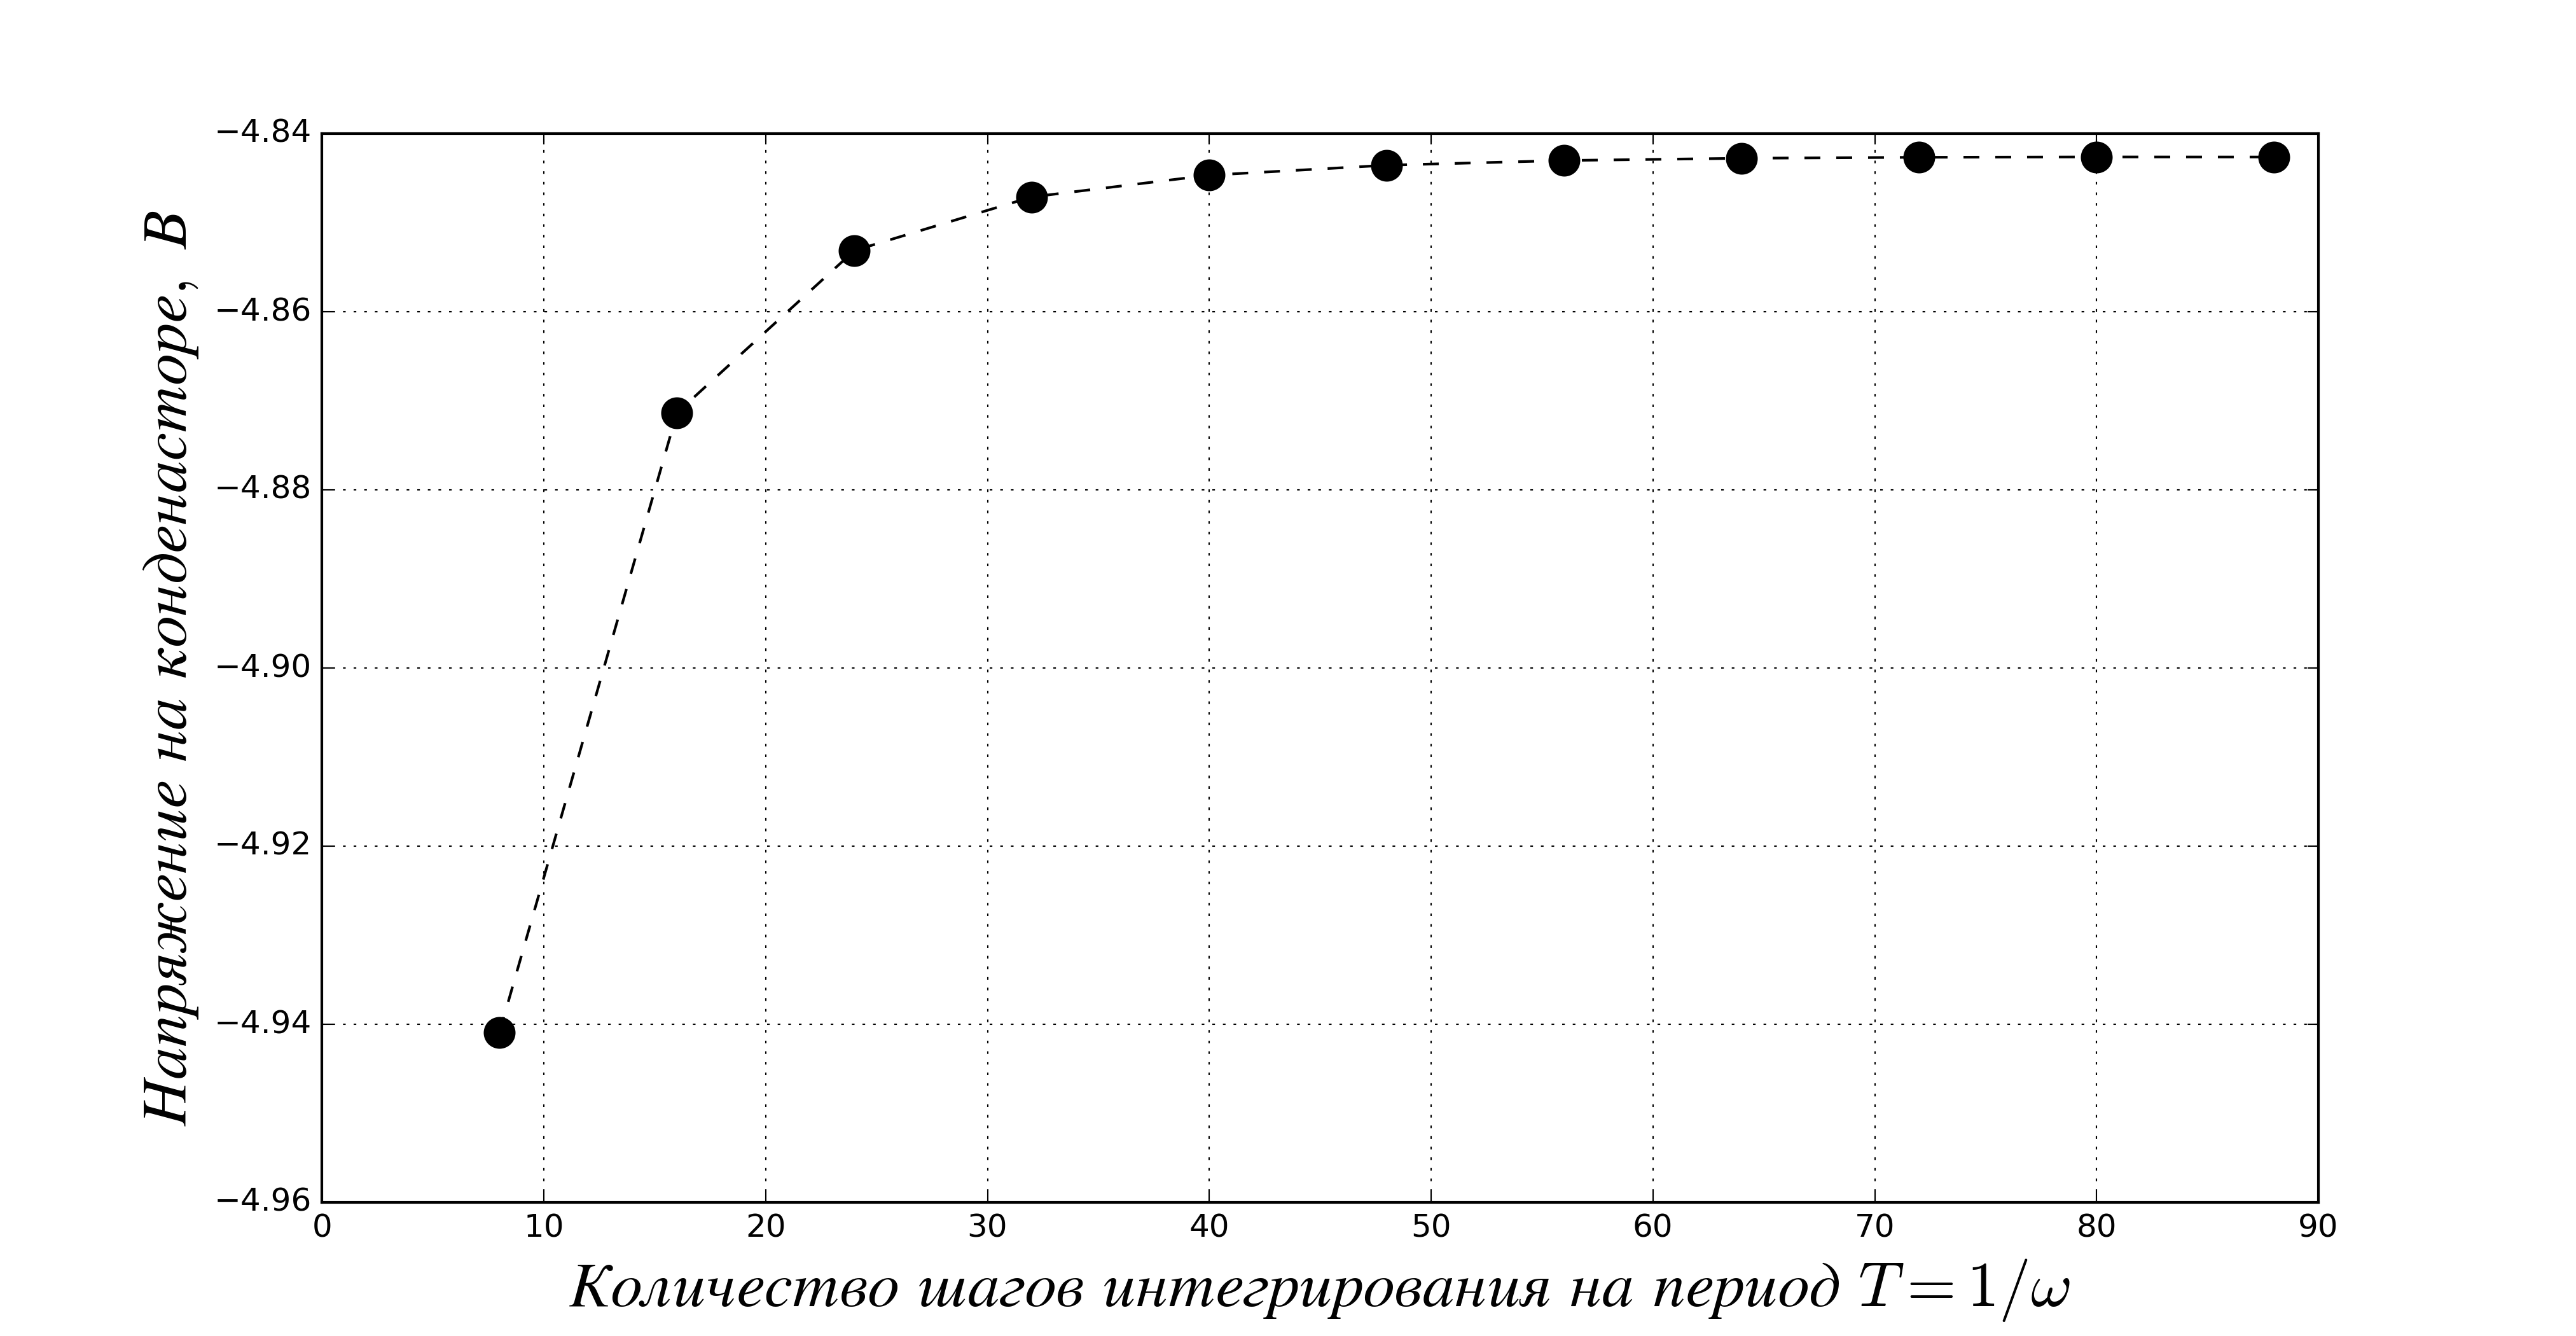
\includegraphics [scale=0.5] {pas_susp_solid226_conv}
  \caption{График сходимости метода прямого решения $y(N)$, где $N$ – количество шагов интегрирования на один период $T=1/\omega$.}
  \label{img:pas_susp_solid226_conv}
\end{figure}

Зададимся точностью $\epsilon = 0.0001$, т.~е. будем считать решение сошедшимся, если угловой коэффициент касательной к графику \ref{img:pas_susp_solid226_conv} не превышает $\epsilon$. Таким образом, минимальное количество шагов интегрирования на один период источника ЭДС необходимое для получения удовлетворяющего принимаем равным $64$, т.~е. $dt_{max}=\frac{1}{64} \cdot T$, где $T = \frac{1}{\omega}$ – период, ${\omega}$ – частота источника напряжения.

Результатом расчета имеем зависимости от времени напряжения на электроде $U$ и электрической силы $F_e$, представленные на рис. \ref{img:pas_susp_solid226_sol}. Отклонение решения методом конечных элементов в модели с 50-ю элементами от прямого численного интегрирования уравнений (\ref{eq:pas_susp_motion}) не превышает $14\%$, а с 500 элементами – $2.3\%$, т.~е. при увеличении плотности разбиения демонстрируется тенденция приближения конечно-элементного решения к некоторому решению, близкому к численно интегрированному уравнению (\ref{eq:pas_susp_motion}). Более подробный анализ сходимости решения от количества разбиений в работе не приведен по причине высокой ресурсоемкости метода.

\begin{figure}[ht] 
  \centering
  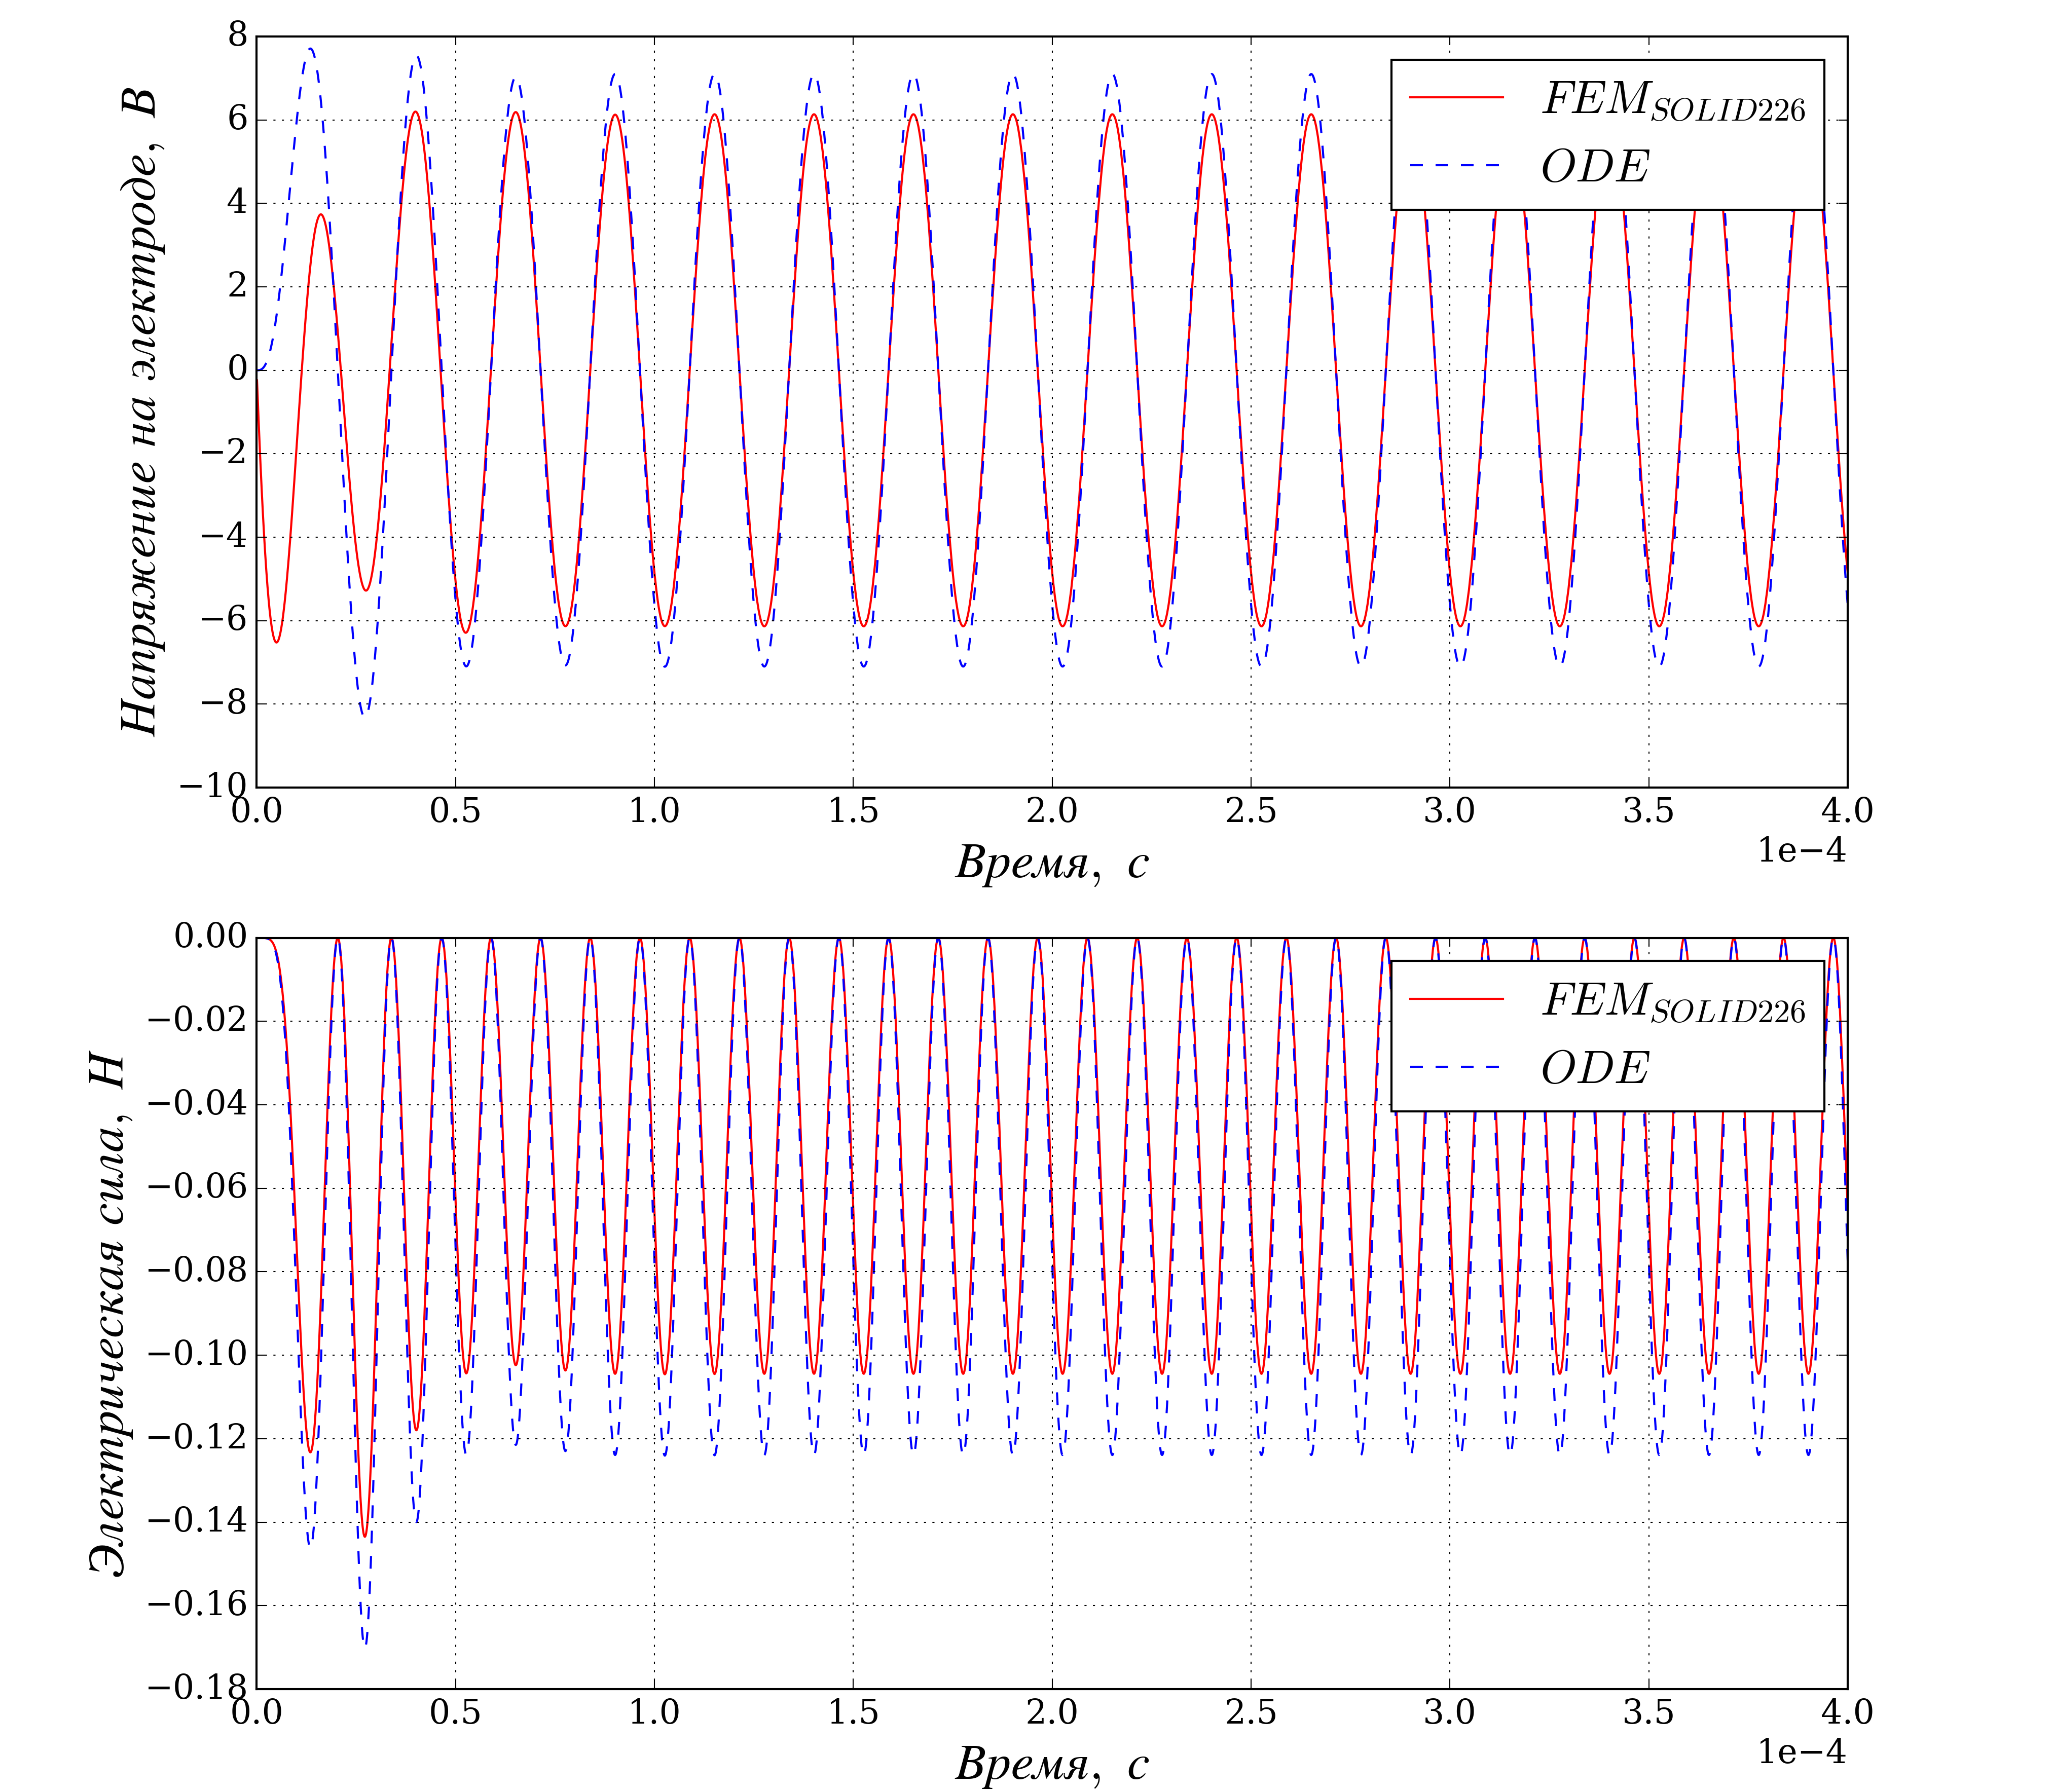
\includegraphics [scale=0.5] {pas_susp_solid226_sol}
  \caption{Результат конечно-элементного расчета методом прямого решения связанной задачи с фиксированным твердом телом в сравнении с численным решением ОДУ (\ref{eq:pas_susp_motion})}
  \label{img:pas_susp_solid226_sol}
\end{figure}

Метод прямого решения связанной задачи требует большого времени счета, что не позволяет выгодно применить его к расчету электромеханической задачи пассивного подвеса со сложной, с точки зрения геометрии, конечно-элементной сетки межэлектродной полостью: зазором $\delta_0 = 3\ \text{мкм}$ при площади $S = 50\ \text{см}^2$. Однако, это не исключает возможности его применения к более простым случаям, более того, метод, как упоминалось ранее, позволяет учитывать неоднородности электрического поля и при этом прост в реализации, что выгодно выделяет его на фоне других подходов.

По этой причине реализуем конечно-элементное решение задачи одноосного пассивного электростатического подвеса с помощью элементов-преобразователей, описанных ранее в разделе \ref{subsect2_2_2}.
Расчетную модель построим путем замыкания в контур 3-х элементов электрической цепи \textit{CIRCU124} и одного электромеханического \textit{TRANS126} элемента. Массу твердого тела, находящегося в пассивном электростатическом подвесе, моделируем \textit{MASS21} элементом. На верхний узел TRANS126, соответствующий верхнему фиксированному электроду, накладываем запрет на перемещение UY $= 0$. На нижний узел накладываем граничное условие первого рода VOLT $= 0$.

\begin{figure}[ht] 
  \centering
  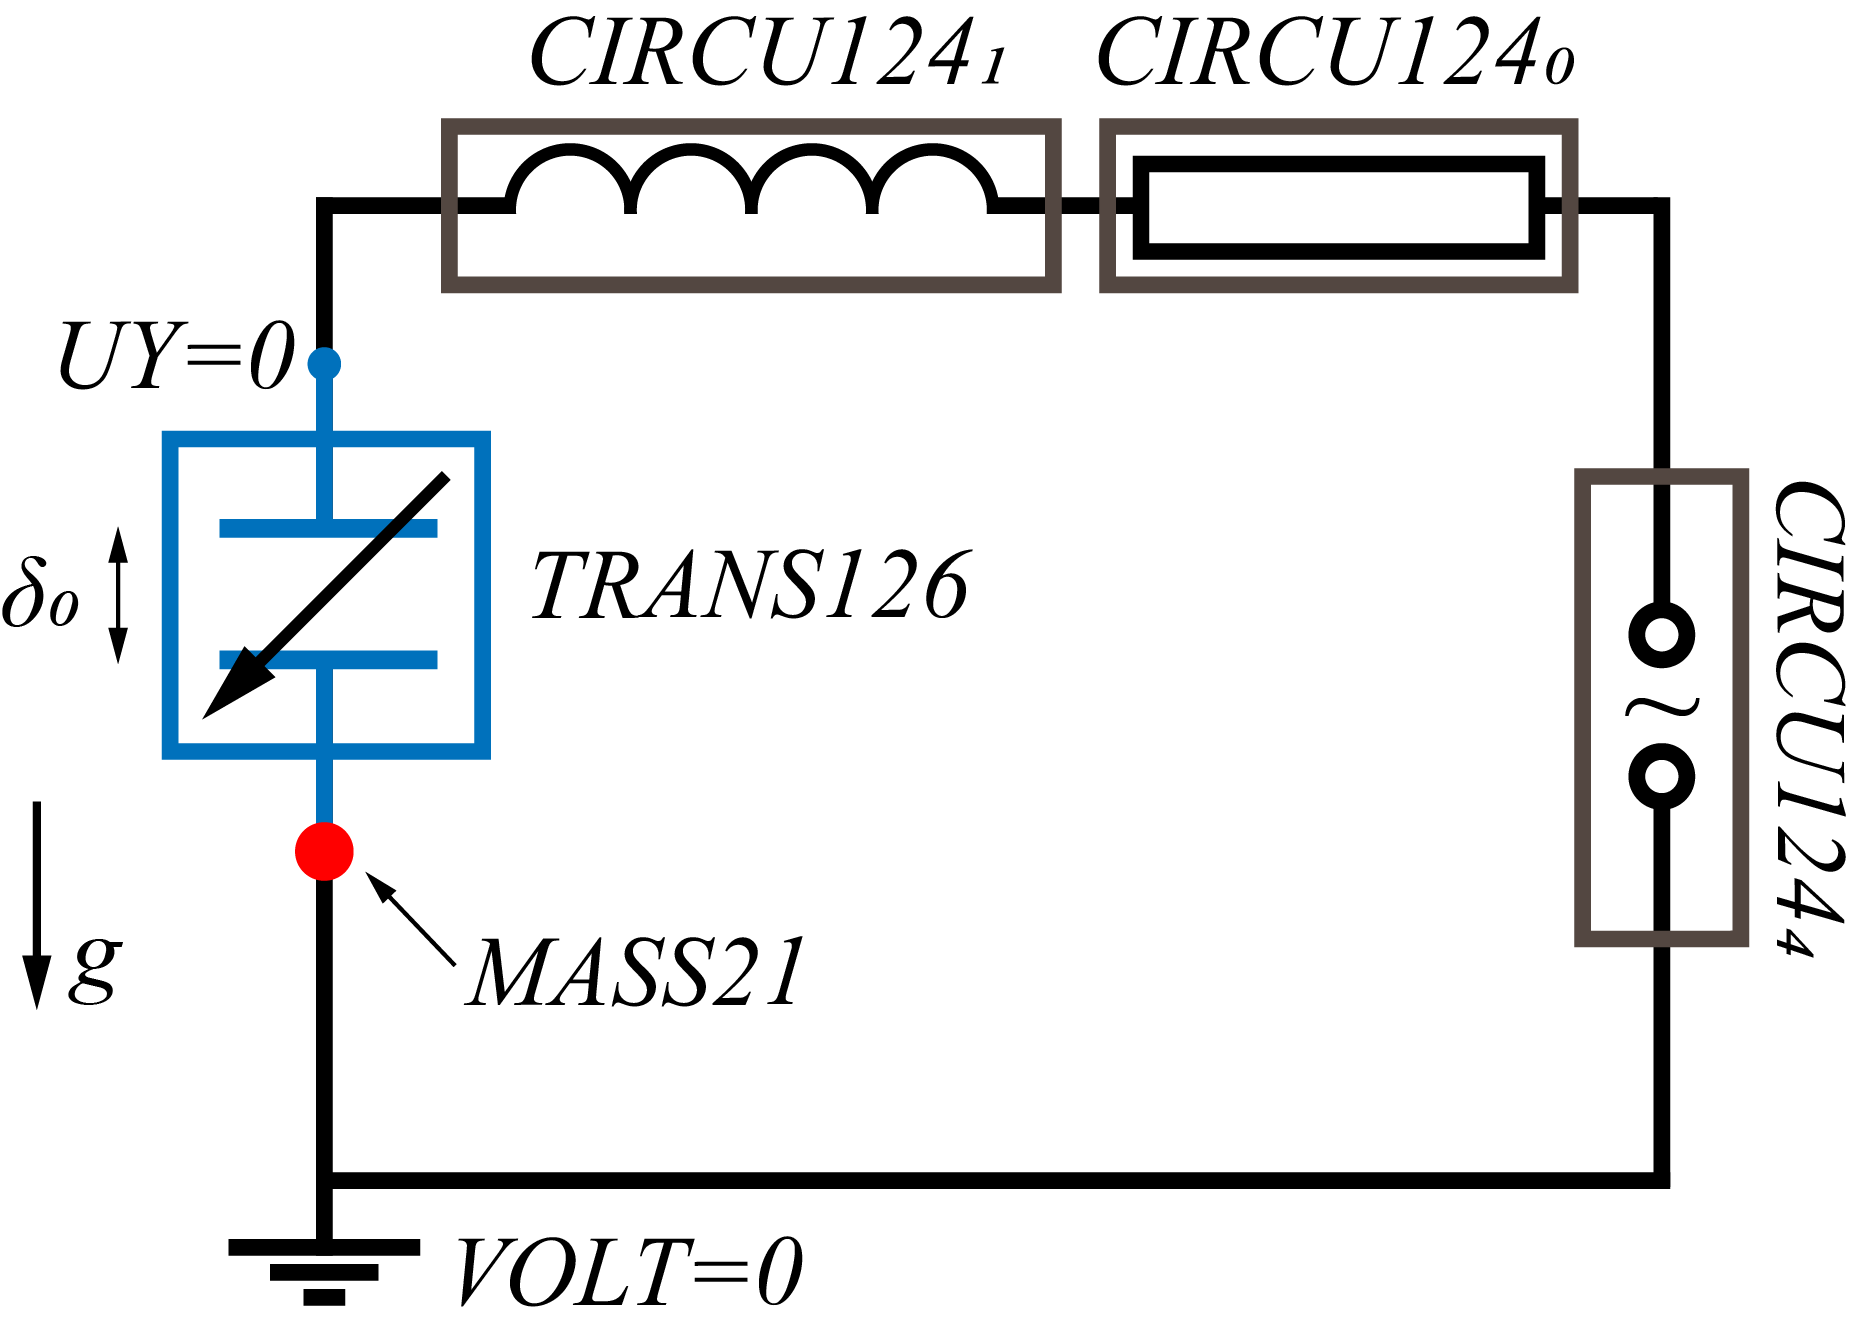
\includegraphics [scale=0.5] {pas_susp_trans126_scheme}
  \caption{Расчетная схема конечно-элементной постановки с использованием электромеханических элементов-преобразователей \textit{TRANS126}}
  \label{img:pas_susp_trans126_scheme}
\end{figure}


Как упоминалось ранее, для функционирования электромеханических элементов TRANS126 необходимо задание в них зависимости электрической емкости от зазора $C(\delta)$, где $\delta = \delta_0 + y_1 - y_2$, $\delta_0$ – номинальный зазор, $y_1, y_2$ – координаты первого и второго узлов элемента. Для расчета электрической емкости используем макрос \textit{CMATRIX}, позволяющий вычислить емкость между двумя фиксированными электродами. Для этого построим конечно-элементную модель эквивалентную конденсатору с площадью обкладок каждого электрода $S = 50\ \text{см}^2$. Для построения модели используем двумерные 8-ми узловые электростатические элементы \textit{PLANE121} с одной степенью свободы VOLT в каждом узле.

Итерационно в 20 шагов (именно столько точек на графике «зазор–емкость» способен хранить элемент) перестраиваем расчетную модель, изменяя на каждом шаге зазор между обкладками, исследуем зависимость электрической емкости от зазора на промежутке $1\ \text{мкм} < \delta < 10\ \text{мкм}$, напомним, что номинальный зазор $\delta_0 = 3\ \text{мкм}$.


\begin{figure}[ht] 
  \centering
  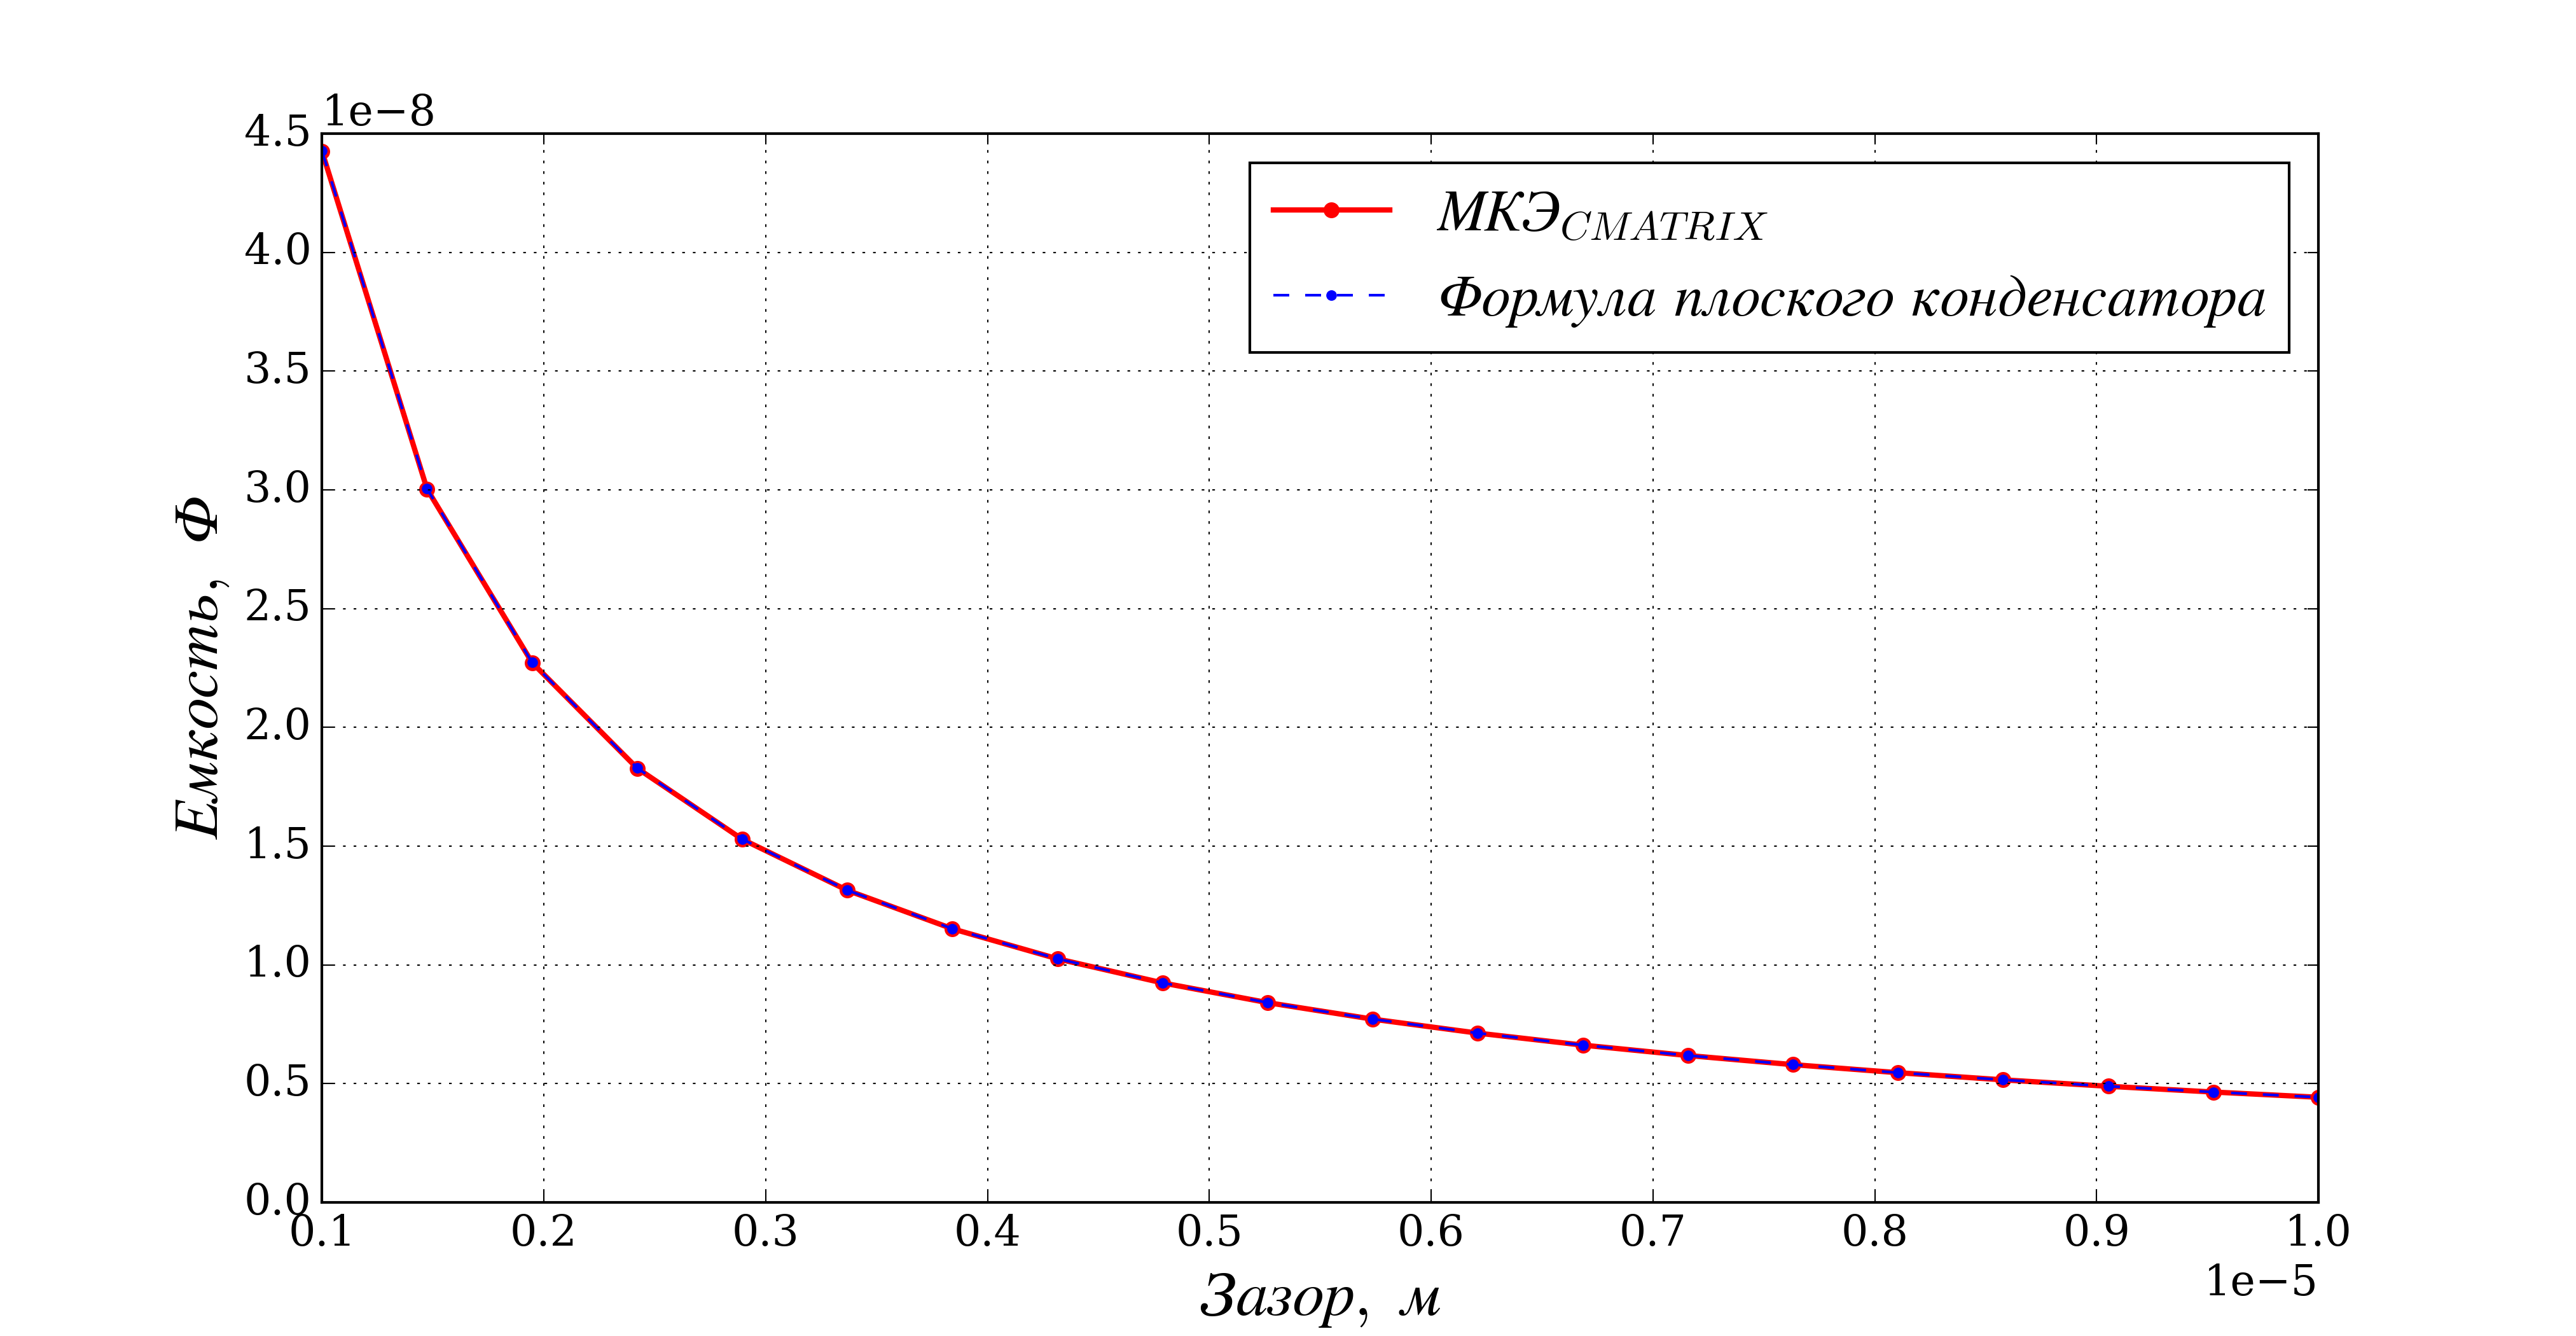
\includegraphics [scale=0.5] {pas_susp_trans126_cap_v_gap}
  \caption{График зависимости емкости от зазора $C(\delta)$, полученной методом конечных элементов, в сравнении с формулой емкости для плоского конденсатора}
  \label{img:pas_susp_trans126_cap_v_gap}
\end{figure}


Результаты динамического анализа расчетной модели методом Ньютона-Рафсона представлены на рис. \ref{img:pas_susp_trans126_sol}.


\begin{figure}[ht] 
  \centering
  \includegraphics [scale=0.5] {pas_susp_trans126_sol}
  \caption{Результат конечно-элементного расчета методом прямого решения связанной задачи с фиксированным твердом телом в сравнении с численным решением ОДУ (\ref{eq:pas_susp_motion})}
  \label{img:pas_susp_trans126_sol}
\end{figure}



\begin{figure}[ht] 
  \centering
  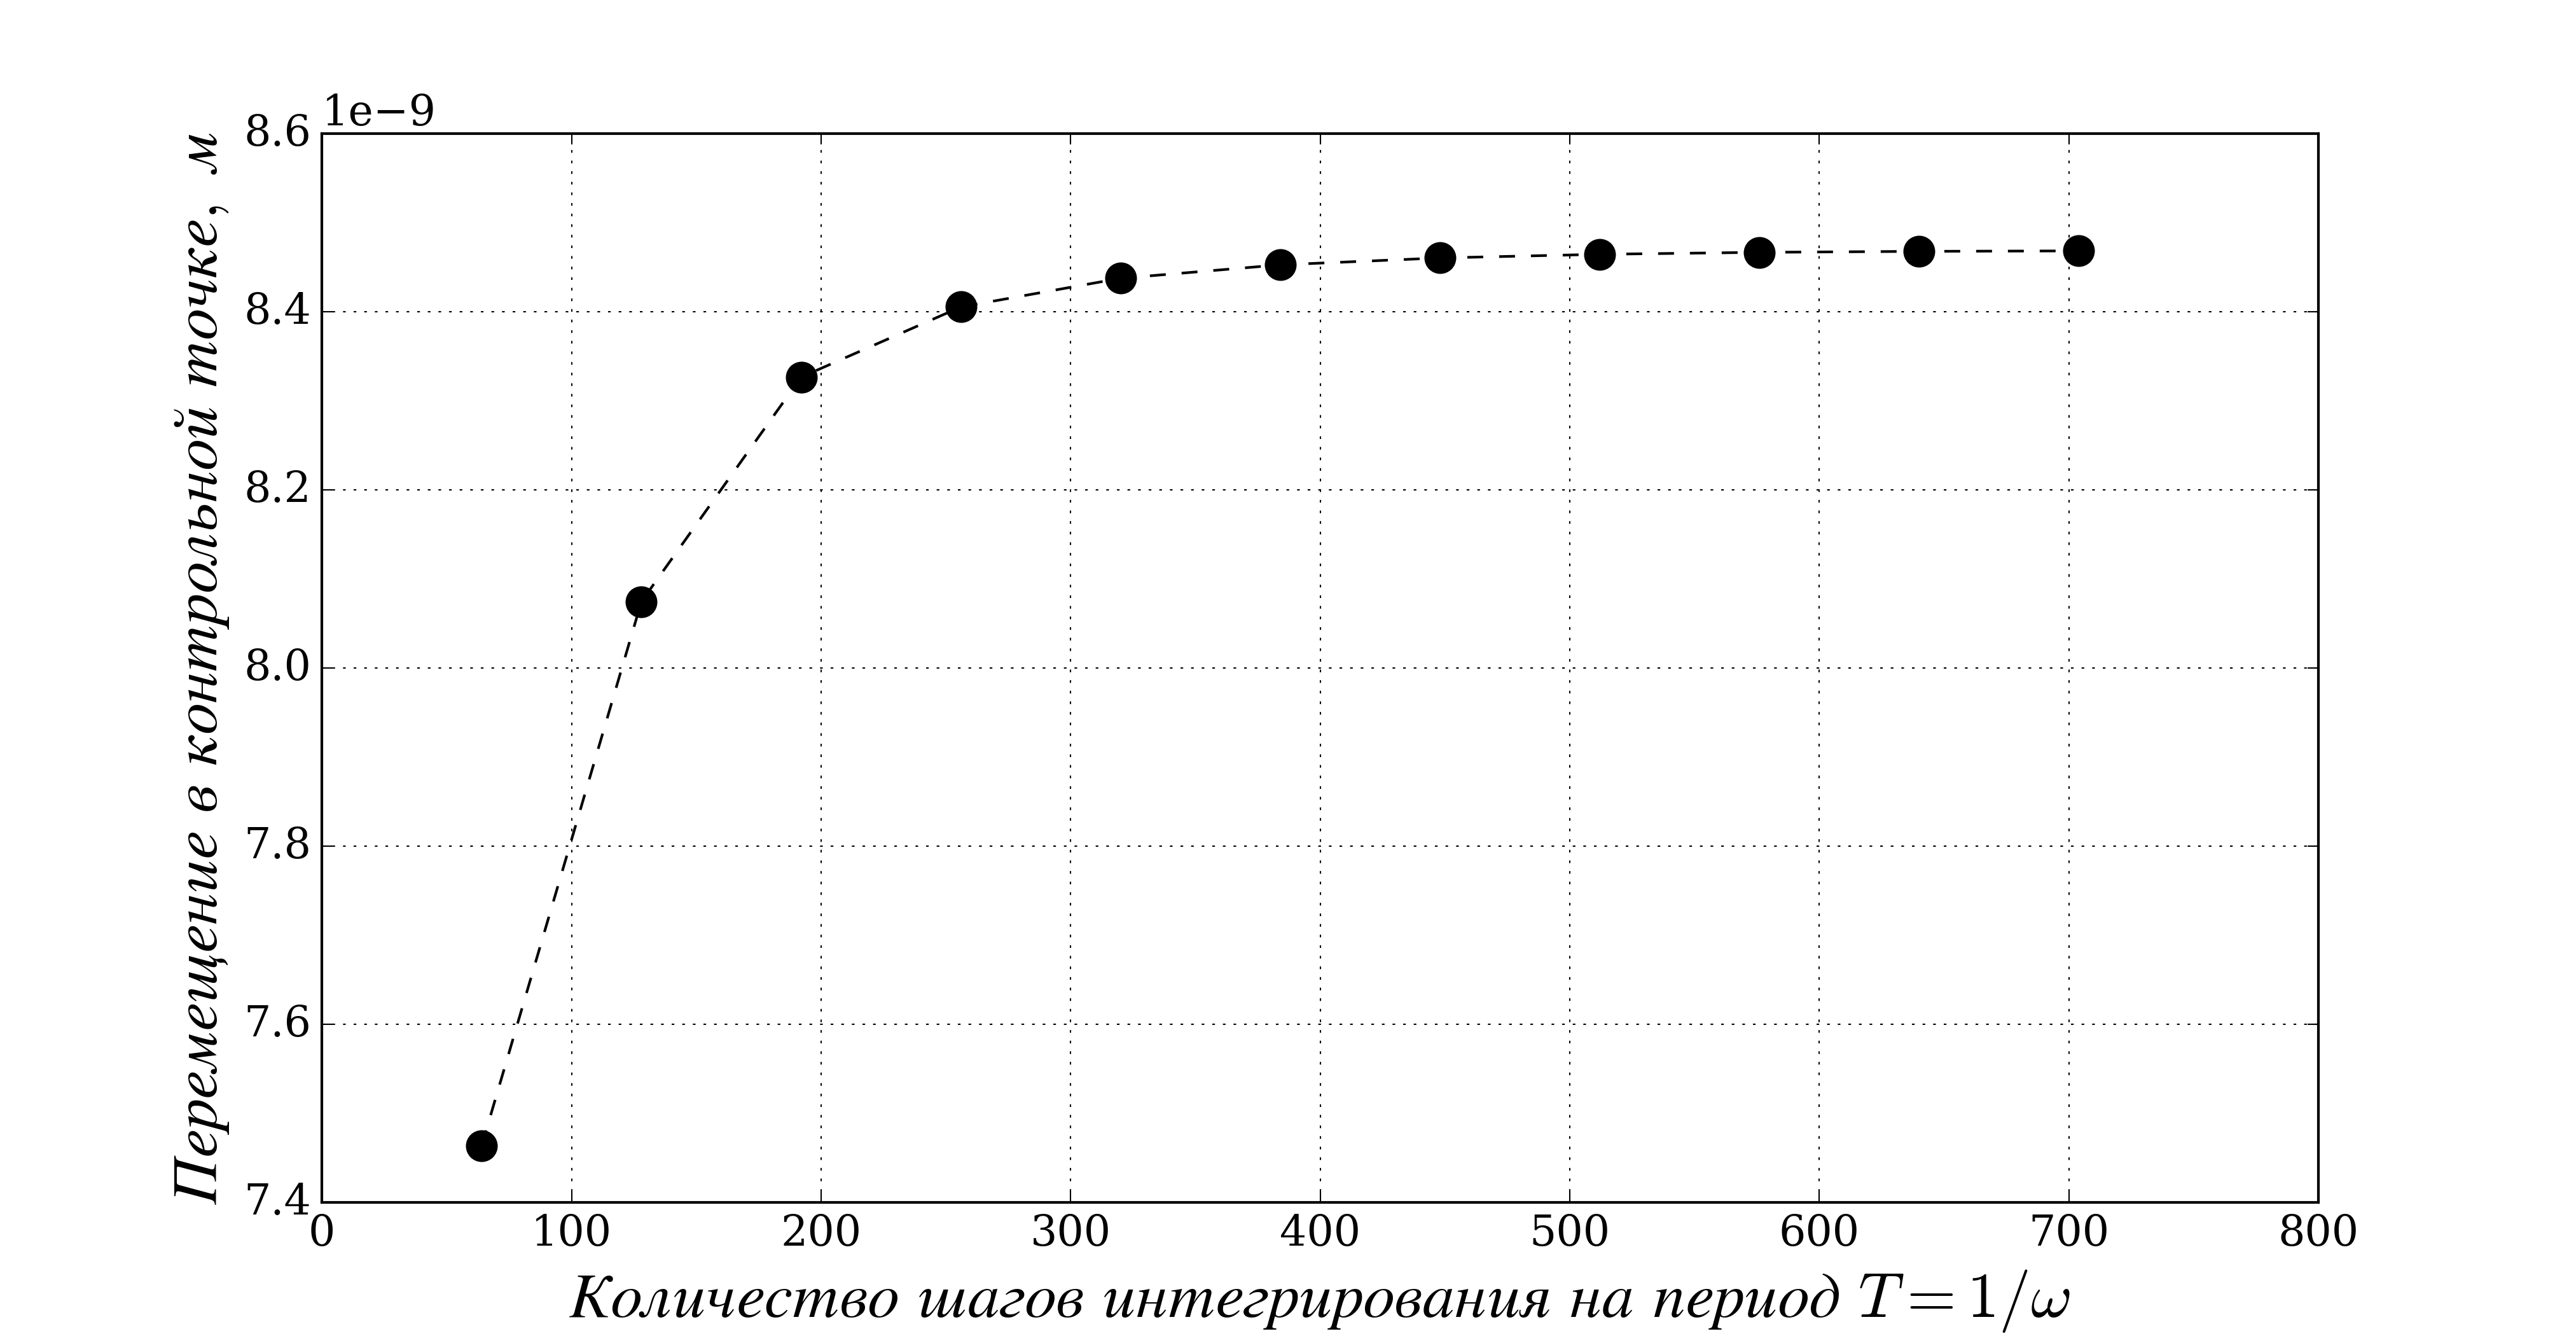
\includegraphics [scale=0.5] {pas_susp_trans126_conv}
  \caption{График сходимости метода с использованием элемента–преобразователя $y(N)$, где $N$ – количество шагов интегрирования на один период $T=1/\omega$.}
  \label{img:pas_susp_trans126_conv}
\end{figure}




%\newpage
%============================================================================================================================
\section{Анализ полученных уравнений методом многих масштабов} \label{sect2_3}


\section{Сравнение результатов в задаче динамики одномерного электрического подвеса с явным моделированием связной задачи в ANSYS}

